%%%%%%%%%%%%%%%%%%%%% {{{
%%Options for presentations (in-class) and handouts (e.g. print).
\documentclass[pdf,9pt]{beamer}
% \documentclass[pdf,9pt]{beamer}


%%%%%%%%%%%%%%%%%%%%%%
%Change this for different slides so it appears in bar
\usepackage{authoraftertitle}
\date{Chapter 2. Matrix Algebra \\ \S 2-6. Linear Transformations}

%%%%%%%%%%%%%%%%%%%%%%
%% Upload common style file
\usepackage{LyryxLAWASlidesStyle}

\begin{document}

%%%%%%%%%%%%%%%%%%%%%%%
%% Title Page and Copyright Common to All Slides

%Title Page
\input frontmatter/titlepage.tex

%LOTS Page
\input frontmatter/lyryxopentexts.tex

%Copyright Page
\input frontmatter/copyright.tex

%%%%%%%%%%%%%%%%%%%%%%%%% }}}

%-------------- start slide -------------------------------%{{{ 2
\begin{frame}[fragile]
   \tableofcontents
\end{frame}
%-------------- end slide -------------------------------%}}}

\section[\textcolor{yellow}{}]{\textcolor{yellow}{Linear Transformations}}

%-------------- start slide -------------------------------%{{{ 3
\frame{
\frametitle{Linear Transformations}
\pause
\begin{definition}
    A transformation $T:\RR^n\rightarrow \RR^m$ is a
    \alert{linear transformation} if it satisfies the following
    two properties for all $\vec{x},\vec{y}\in\RR^n$ and all (scalars) $a\in\RR$.
    \pause
    \begin{enumerate}
	\item $T(\vec{x}+\vec{y})=T(\vec{x})+T(\vec{y})$ \hfill\alert{(preservation of addition)}
	    \pause
	\item $T(a\vec{x})=aT(\vec{x})$ \hfill\alert{(preservation of scalar multiplication)}
    \end{enumerate}
\end{definition}
}
%-------------- end slide -------------------------------%}}}

%-------------- start slide -------------------------------%{{{ 4
\frame{
\begin{emptytitle}
    % \begin{center}
	% \textcolor{yellow}{Properties of Linear Transformations}
    % \end{center}
    Let $T:\RR^n\to\RR^m$ be a linear transformation, and
    let $\vec{x}\in\RR^n$.
    \pause
    Since $T$ preserves scalar multiplication,
    \begin{enumerate}
    \pause
    \item $T(0\vec{x})=0T(\vec{x})$ implying $T(\vec{0})=\vec{0}$, so \alert{$T$ preserves the zero vector}.
    \pause
    \item $T((-1)\vec{x})=(-1)T(\vec{x})$, implying $T(-\vec{x})=-T(\vec{x})$,
    so \alert{$T$ preserves the negative of a vector}.
    \end{enumerate}
    \vspace{2em}
    \pause
    Suppose $\vec{x}_1, \vec{x}_2, \ldots, \vec{x}_k$ are vectors in $\RR^n$
    and for some $a_1, a_2, \ldots, a_k\in\RR$.
    \[ \vec{y} = a_1\vec{x}_1 + a_2\vec{x}_2 +\cdots + a_k\vec{x}_k.\]
    \pause
    \vspace{-1em}
    \[\Downarrow\]
    \vspace{-2em}
    \begin{enumerate}
    \setcounter{enumi}{2}
    \item
    \[ \begin{array}{rcl}
    T(\vec{y}) & = & T(a_1\vec{x}_1 + a_2\vec{x}_2 +\cdots + a_k\vec{x}_k) \\
    & = & a_1T(\vec{x}_1) + a_2T(\vec{x}_2)+\cdots + a_kT(\vec{x}_k),
    \end{array}\]
    i.e., \alert{$T$ preserves linear combinations.}
    \end{enumerate}
\end{emptytitle}
}
%-------------- end slide -------------------------------%}}}

%-------------- start slide -------------------------------%{{{ 5
\frame{
\begin{problem}
    Let $T:\RR^3 \rightarrow \RR^4$ be a linear transformation
    such that
    \[ T\left[\begin{array}{r}
	    1 \\ 3 \\ 1
    \end{array}\right]
    =
    \left[\begin{array}{r}
	    4 \\ 4\\ 0 \\ -2
    \end{array}\right]
    \quad\text{and}\quad
    T\left[\begin{array}{r}
	    4 \\ 0 \\ 5
    \end{array}\right]
    =
    \left[\begin{array}{r}
	    4 \\ 5 \\ -1 \\ 5
    \end{array}\right].
    \pause
    \mbox{ Find }
    T\left[\begin{array}{r}
	    -7 \\ 3 \\ -9
    \end{array}\right].\]
\end{problem}
\pause
\vfill
\begin{solution}
    The only way it is possible to solve this problem is if
    \[ \left[\begin{array}{r}
	    -7 \\ 3 \\ -9
    \end{array}\right]
    \mbox{ is a linear combination of }
    \left[\begin{array}{r}
	    1 \\ 3 \\ 1
    \end{array}\right]
    \quad\text{and}\quad
    \left[\begin{array}{r}
	    4 \\ 0 \\ 5
    \end{array}\right],\]
    % \vspace*{-.1in}

    \pause
    i.e., if there exist $a,b\in\RR$ so that
    % \vspace*{-.1in}

    \[ \left[\begin{array}{r}
	    -7 \\ 3 \\ -9
    \end{array}\right]
    =
    a\left[\begin{array}{r}
	    1 \\3 \\ 1
    \end{array}\right]
    +
    b\left[\begin{array}{r}
	    4 \\ 0 \\ 5
    \end{array}\right].
\]
\end{solution}
}
%-------------- end slide -------------------------------%}}}

%-------------- start slide -------------------------------%{{{ 6
\frame{
\begin{solution}[continued]
    To find $a$ and $b$, solve the system of three
    equations in two variables:
    \[
	\left[\begin{array}{rr|r}
		1 & 4 & -7 \\
		3 & 0 & 3 \\
		1 & 5 & -9
	\end{array}\right]
	\rightarrow \cdots \rightarrow
	\left[\begin{array}{rr|r}
		1 & 0 & 1 \\
		0 & 1 & -2 \\
		0 & 0 & 0
	\end{array}\right]
    \]
    Thus $a=1$, $b=-2$, and
    \[ \left[\begin{array}{r}
	    -7 \\ 3 \\ -9
    \end{array}\right]
    =
    \left[\begin{array}{r}
	    1 \\ 3 \\ 1
    \end{array}\right]
    -
    2\left[\begin{array}{r}
	    4 \\ 0 \\ 5
    \end{array}\right].
\]
\end{solution}
}
%-------------- end slide -------------------------------%}}}

%-------------- start slide -------------------------------%{{{ 7
\frame{
\begin{solution}[continued]
    We now use that fact that linear transformations preserve
    linear combinations, implying that
    \begin{eqnarray*}
	T \left[\begin{array}{r}
		-7 \\ 3 \\ -9
	\end{array}\right]
	& = &
	T\left(
	\left[\begin{array}{r}
		1 \\ 3 \\ 1
	\end{array}\right]
	-
	2\left[\begin{array}{r}
		4 \\ 0 \\ 5
	\end{array}\right]\right)\\
	\pause
	& = &
	T \left[\begin{array}{r}
	    1 \\ 3 \\ 1
	\end{array}\right]
	- 2T\left[\begin{array}{r}
	    4 \\ 0 \\ 5
	\end{array}\right] \\
	\pause
	& = &
	\left[\begin{array}{r}
	    4 \\ 4 \\ 0 \\ -2
	\end{array}\right]
	- 2\left[\begin{array}{r}
	    4 \\ 5 \\ -1 \\ 5
	\end{array}\right]
	=
	\left[\begin{array}{r}
	    -4 \\ -6 \\ 2 \\ -12
	\end{array}\right]
    \end{eqnarray*}
    \pause
    Therefore,
    $T \left[\begin{array}{r}
	    -7 \\ 3 \\ -9
    \end{array}\right]
    = \left[\begin{array}{r}
	    -4 \\ -6 \\ 2 \\ -12
    \end{array}\right]$.
    \myQED
\end{solution}
}
%-------------- end slide -------------------------------%}}}

%-------------- start slide -------------------------------%{{{ 8
\frame{
\begin{problem}
    Let $T:\RR^4 \rightarrow \RR^3$ be a linear transformation
    such that
    \[ T\left[\begin{array}{r}
	    1\\1\\ 0 \\ -2
    \end{array}\right]
    =
    \left[\begin{array}{r}
	    2 \\ 3 \\ -1
    \end{array}\right]
    \quad\text{and}\quad
    T\left[\begin{array}{r}
	    0\\-1 \\ 1 \\ 1
    \end{array}\right]
    =
    \left[\begin{array}{r}
	    5 \\ 0 \\ 1
    \end{array}\right].
    \mbox{ Find }
    T\left[\begin{array}{r}
	    1 \\ 3 \\ -2\\-4
    \end{array}\right].\]
\end{problem}
\pause
\vfill
\begin{solution}[ Final Answer ]
    \[ T\left[\begin{array}{r}
	    1 \\ 3 \\ -2\\-4
    \end{array}\right]
    =\left[\begin{array}{r}
	    -8 \\ 3 \\ -3
    \end{array}\right].\]
    \myQED
\end{solution}
}
%-------------- end slide -------------------------------%}}}

%-------------- start slide -------------------------------%{{{ 9
\frame{
\begin{theorem}
    Every matrix transformation is a linear transformation.
\end{theorem}
\pause
\pause
\begin{proofnoend}
    Suppose $T:\RR^n\rightarrow\RR^m$ is a matrix transformation
    induced by the $m\times n$ matrix $A$,
    \pause
    i.e., $T(\vec{x})=A\vec{x}$ for each $\vec{x}\in\RR^n$.
    \pause
    Let $\vec{x},\vec{y}\in\RR^n$ and let $a\in\RR$.
    \pause
    Then
    \[ T(\vec{x}+\vec{y})=A(\vec{x}+\vec{y})=A\vec{x}+A\vec{y}=T(\vec{x})+T(\vec{y}),\]
    \pause
    proving that $T$ preserves addition.
    \pause
    Also,
    \pause
    \[ T(a\vec{x})=A(a\vec{x})=a(A\vec{x})=aT(\vec{x}),\]
    \pause
    proving that $T$ preserves scalar multiplication.
    \pause
    \bigskip

    Since $T$ preserves addition and scalar multiplication
    $T$ is a linear transformation.
    \myQED
\end{proofnoend}
}
%-------------- end slide -------------------------------%}}}

%-------------- start slide -------------------------------%{{{ 10
\frame{
\begin{example}[The Zero Transformation]
    If $A$ is the $m \times n$ matrix of zeros,
    then the transformation $T:\RR^n\to\RR^m$ induced by $A$
    is called the \alert{zero transformation} because
    for every vector $\vec{x}$ in $\RR^n$
    \[ T(\vec{x}) = A\vec{x} = O\vec{x} = \vec{0}. \]
    \pause
    The zero transformation is usually written as \alert{$T=0$}.
\end{example}
\pause
\vfill
\begin{example}[The Identity Transformation]
The transformation of $\RR^n$ induced by $I_n$, the
$n\times n$ identity matrix,
is called the \alert{identity transformation}
because for every vector $\vec{x}$ in $\RR^n$,
\[ T(\vec{x}) = I_n\vec{x}=\vec{x}.  \]
\pause
The identity transformation on $\RR^n$ is usually written
as \alert{$1_{\RR^n}$}.
\end{example}
}
%-------------- end slide -------------------------------%}}}

%-------------- start slide -------------------------------%{{{ 11
\begin{frame}[fragile]
\begin{problem}[Revisited]
    Is the following $T:\RR^3\rightarrow\RR^4$ a matrix transformation?
    \[
	T\left[\begin{array}{c} a \\ b\\ c\end{array}\right]
	=\left[ \begin{array}{c}
	a+b \\ b+c \\ a-c\\ c-b \end{array}\right]
    \]
\end{problem}
\vfill
\pause
\begin{solution}
  %   Consider $A=
  %   \left[ \begin{array}{rrr}
	%     1 & 1 & 0 \\
	%     0 & 1 & 1 \\
	%     1 & 0 & -1 \\
	%     0 & -1 & 1 \\
	% \end{array}
  %   \right]$, then
  %
\[
	A\left[\begin{array}{r} a \\ b\\ c \end{array}\right]
	=
	\left[ \begin{array}{rrr}
		1 & 1 & 0 \\
		0 & 1 & 1 \\
		1 & 0 & -1 \\
		0 & -1 & 1 \\
	    \end{array}
	\right]
	\left[\begin{array}{r} a \\ b\\ c \end{array}\right]
	=
	\left[ \begin{array}{c}
	a+b \\ b+c \\ a-c\\ c-b \end{array}\right]
	=
	T\left[\begin{array}{c} a \\ b\\ c\end{array}\right]
   \]
    \pause
    Yes, $T$ is a matrix transformation.
    \myQED
\end{solution}
\end{frame}
%-------------- end slide -------------------------------%}}}

%-------------- start slide -------------------------------%{{{ 12
\frame{
\begin{problem}[Not all transformations are matrix transformations]
    Consider $T:\RR^2 \rightarrow \RR^2$ defined by
    \[ T(\vec{x}) = \vec{x} +
    \left[\begin{array}{r} 1 \\ -1 \end{array}\right]
    \mbox{ for all } \vec{x}\in\RR^2.\]
    Show that  $T$ NOT a matrix transformation.
\end{problem}
}
%-------------- end slide -------------------------------%}}}

%-------------- start slide -------------------------------%{{{ 13
\frame{
\begin{solution}
    We have $T:\RR^2 \rightarrow \RR^2$ defined by
    \[ T(\vec{x}) = \vec{x} +
    \left[\begin{array}{r} 1 \\ -1 \end{array}\right]
    \mbox{ for all } \vec{x}\in\RR^2.\]
    \pause

    Since every matrix transformation is a linear transformation,
    \pause
    we consider $T(0)$, where $0$ is the zero vector of $\RR^2$.
    \pause
    \[ T\left[\begin{array}{r} 0 \\ 0 \end{array}\right] \pause
    = \left[\begin{array}{r} 0 \\ 0 \end{array}\right]
    +
    \left[\begin{array}{r} 1 \\ -1 \end{array}\right]
    \pause
    = \left[\begin{array}{r} 1 \\ -1 \end{array}\right]
    \pause
    \neq  \left[\begin{array}{r} 0 \\ 0 \end{array}\right],\]
    violating one of the properties of a linear transformation.
    \pause
    \bigskip

    Therefore, $T$ is not a linear transformation, and hence is
    not a matrix transformation.
    \myQED
\end{solution}
}
%-------------- end slide -------------------------------%}}}

%-------------- start slide -------------------------------%{{{ 15
\frame{
\begin{remark}
    Recall that a transformation $T:\RR^n\rightarrow \RR^m$ is a
    \alert{linear transformation} if it satisfies the following
    two properties for all $\vec{x},\vec{y}\in\RR^n$ and all (scalars) $a\in\RR$.
    \pause
    \begin{enumerate}
    \item $T(\vec{x}+\vec{y})=T(\vec{x})+T(\vec{y})$ \hfill\alert{(preservation of addition)}
	\pause
    \item $T(a\vec{x})=aT(\vec{x})$ \hfill\alert{(preservation of scalar multiplication)}
    \end{enumerate}
\end{remark}
\vfill
\pause
\begin{theorem}[Every Linear Transformation is a Matrix Transformation]
    Let $T:\RR^n\rightarrow\RR^m$ be a linear transformation. Then we can find an $n \times m$ matrix $A$ such that
    \[
	T(\vec{x})=A\vec{x}
    \]
    \pause
    In this case, we say that $T$ is induced, or determined, by $A$ and we write
    \[
	T_A(\vec{x}) = A\vec{x}
    \]
\end{theorem}
\bigskip
\begin{center}
    ``linear" = ``matrix"
\end{center}
}
%-------------- end slide -------------------------------%}}}

%-------------- start slide -------------------------------%{{{ 16
\frame{
\begin{problem}
    The transformation
    $T:\RR^3\rightarrow\RR^4$ defined by
    \begin{align*}
        T\left[\begin{array}{c} a \\ b\\ c\end{array}\right]
        =\left[ \begin{array}{c}
        a+b \\ b+c \\ a-c\\ c-b \end{array}\right]
    \end{align*}
    for each $\vec{x}\in\RR^3$
    is another matrix transformation, that is,
    $T(\vec{x}) = A\vec{x}$ for some matrix $A$.
    \alert{Can you find a matrix $A$ that works?}
\end{problem}
\pause
\vfill
}
%-------------- end slide -------------------------------%}}}

%-------------- start slide -------------------------------%{{{ 17
\frame{
\begin{solution}
    First, since $T:\RR^3\to\RR^4$, we know that $A$ must have size
    \pause
    \alert{$4\times 3$}.
    \pause
    Now consider the product
    \[ \left[\begin{array}{rrr}
	? & ? & ? \\
	? & ? & ? \\
	? & ? & ? \\
	? & ? & ?
    \end{array}\right]
    \left[\begin{array}{c} a \\ b \\ c \end{array}\right] =
    \left[\begin{array}{c} a+b \\ b+c \\ a-c \\ c-b \end{array}\right],
    \]
    and try to fill in the values of the matrix.
    \pause
    \bigskip
    \[\vdots\]

    We can deduce from the product that $T$ is induced by
    the matrix
    \[ A=\left[\begin{array}{rrr}
    1 & 1 & 0 \\ 0 & 1 & 1 \\ 1 & 0 & -1 \\
    0 & -1 & 1 \end{array}\right]. \]
    \myQED
\end{solution}
}
%-------------- end slide -------------------------------%}}}

\section[\textcolor{yellow}{}]{\textcolor{yellow}{Finding the Matrix of a Linear Transformation}}

%-------------- start slide -------------------------------%{{{ 18
\frame{
\frametitle{Finding the Matrix of a Linear Transformation}
\pause
\begin{emptytitle}
    Is there an easier way to find the matrix of $T$?
    \pause
    For some transformations guess and check will work, but this is not an efficient method. The
    next theorem gives a method for finding the matrix of $T$.
\end{emptytitle}
\vfill
\pause
\begin{definition}
    The set of columns $\{ \vec{e}_1, \vec{e}_2, \ldots, \vec{e}_n\}$ of $I_n$ is
    called the \alert{standard basis of $\RR^n$.}
\end{definition}
}
%-------------- end slide -------------------------------%}}}

%-------------- start slide -------------------------------%{{{ 19
\frame{
\begin{theorem}[Matrix of a Linear Transformation]
    Let $T:\RR^n\rightarrow \RR^m$ be a linear transformation.
    \pause
    Then $T$ is a matrix transformation.
    \pause
    Furthermore,
    $T$ is induced by the
    \alert{unique} matrix
    \[ A =
    \left[\begin{array}{cccc}
    T(\vec{e}_1) & T(\vec{e}_2) & \cdots & T(\vec{e}_n) \end{array}\right],
    \]
    where $\vec{e}_j$ is the $j$-th column of $I_n$,
    and $T(\vec{e}_j)$ is the $j$-th column of $A$.
\end{theorem}
\pause
\vfill
\begin{corollary}
    A transformation $T:\RR^n\rightarrow \RR^m$ is a linear transformation if and only if it is a matrix transformation.
\end{corollary}
\bigskip
\begin{center}
    ``linear" = ``matrix"
\end{center}
}
%-------------- end slide -------------------------------%}}}

%-------------- start slide -------------------------------%{{{ 20
\frame{
    \begin{problem}
        Let $T:\RR^2\to\RR^2$ be a linear transformation defined by
        \[ T \left[ \begin{array}{c} x \\ y \end{array} \right]
        =
        \left[ \begin{array}{c} x+ 2y \\ x - y \end{array} \right]
    \]
    for each $\vec{x}\in\RR^2$.
    Find the matrix, $A$, of $T$.
\end{problem}
\pause
\vfill
\begin{solution}
    \[
        T\left[ \begin{array}{r} 1 \\ 0 \end{array} \right] \pause
        = \left[ \begin{array}{c} 1 + 2(0) \\ 1-0 \end{array} \right] \pause
        = \left[ \begin{array}{r} \textcolor{red}{1} \\ \textcolor{red}{1} \end{array} \right] \pause \quad\text{and}\quad
        T\left[ \begin{array}{r} 0 \\ 1 \end{array} \right] \pause
        = \left[ \begin{array}{c} 0 + 2(1) \\ 0-1 \end{array} \right] \pause
        = \left[ \begin{array}{r} \textcolor{blue}{2} \\ \textcolor{blue}{-1} \end{array} \right]
    \]
    \pause
    \[\Downarrow\]

    \[ A = \left[ \begin{array}{rr}
            \textcolor{red}{1} & \textcolor{blue}{2} \\
            \textcolor{red}{1} &\textcolor{blue}{-1}
    \end{array} \right] \]
    \myQED
\end{solution}
}
%-------------- end slide -------------------------------%}}}

%-------------- start slide -------------------------------%{{{ 21
\frame{
\begin{emptytitle}
   Sometimes, $T$ is defined through its actions several concrete vectors.
\end{emptytitle}
\vfill

\begin{problem}
    Find the matrix $A$ of $T$ where $T$ is given as
    \[ T\left[
    \begin{array}{r}
    1 \\
    1
    \end{array}
    \right] =\left[
    \begin{array}{r}
    1 \\
    2
    \end{array}
    \right]
    \quad\text{and}\quad
    T\left[
    \begin{array}{r}
    0 \\
    -1
    \end{array}
    \right] =\left[
    \begin{array}{r}
    3 \\
    2
    \end{array}
    \right].
    \]
\end{problem}
}
%-------------- end slide -------------------------------%}}}

%-------------- start slide -------------------------------%{{{ 22
\frame{
\begin{solution}[continued]
    We need to write $\vec{e}_1$ and $\vec{e}_2$ as a linear combination of the vectors provided.
    First, find $x$ and $y$ such that
    \[
    \left[
    \begin{array}{r}
    1 \\
    0
    \end{array}
    \right] = x\left[
    \begin{array}{r}
    1\\
    1
    \end{array}
    \right] +y\left[
    \begin{array}{r}
    0 \\
    -1
    \end{array}
    \right]
    \]

    \pause
    Once we find $x$ and $y$ we can compute
    \[
    T\left[
    \begin{array}{r}
    1 \\
    0
    \end{array}
    \right]  = x T\left[
    \begin{array}{r}
    1 \\
    1
    \end{array}
    \right] +y T\left[
    \begin{array}{r}
    0 \\
    -1
    \end{array}
    \right]
    \]
    \[
    =
     x\left[
    \begin{array}{r}
    1 \\
    2
    \end{array}
    \right] +y\left[
    \begin{array}{r}
    3 \\
    2
    \end{array}
    \right]
    \]
\end{solution}
}
%-------------- end slide -------------------------------%}}}

%-------------- start slide -------------------------------%{{{ 23
\frame{
\begin{solution}[continued]
    Finding $x$ and $y$ involves solving the following system of equations.
    \[
    \begin{array}{c}
    x = 1 \\
    x - y = 0
    \end{array}
    \]

    \pause
    The solution is $x=1, y=1$. \pause Hence, we can find $T(\vec{e}_1)$ as follows.
    \[
    T\left[
    \begin{array}{r}
    1 \\
    0
    \end{array}
    \right] =
     1 \left[
    \begin{array}{r}
    1 \\
    2
    \end{array}
    \right] + 1 \left[
    \begin{array}{r}
    3 \\
    2
    \end{array}
    \right]
    =
     \left[
    \begin{array}{r}
    1 \\
    2
    \end{array}
    \right] + \left[
    \begin{array}{r}
    3 \\
    2
    \end{array}
    \right]
    =
    \left[
    \begin{array}{r}
        \textcolor{blue}{4} \\
        \textcolor{blue}{4}
    \end{array}
    \right].
    \]
    As for $T(\vec{e}_2)$,
    \[
    T\left[
    \begin{array}{r}
    0 \\
    1
    \end{array}
    \right]
    =
    -T\left[
    \begin{array}{r}
    0 \\
    -1
    \end{array}
    \right] =
    \left[
    \begin{array}{r}
        \textcolor{red}{-3} \\
        \textcolor{red}{-2}
    \end{array}
    \right].
    \]
    \[\Downarrow\]
    \[
    A
    =
    \left[
    \begin{array}{rr}
        \textcolor{blue}{4} & \textcolor{red}{-3} \\
        \textcolor{blue}{4} & \textcolor{red}{-2}
    \end{array}
    \right]
    \]
    \myQED
\end{solution}
}
%-------------- end slide -------------------------------%}}}

%-------------- start slide -------------------------------%{{{ 24
\frame{
\begin{problem}
    Let $T:\RR^2\rightarrow\RR^3$ be a transformation defined by
    $T\left[\begin{array}{c} x \\ y \end{array}\right] =
    \left[\begin{array}{c} 2x \\ y \\ -x +2y \end{array}\right]$.
    Is $T$ a linear transformation?
\end{problem}
\pause
\vfill
\begin{solution}
    If $T$ were a linear transformation, then $T$ would be induced by the matrix
    \pause
    \[ A= \left[ \begin{array}{cc} T(\vec{e}_1) & T(\vec{e}_2)
    \end{array}\right]
    \pause
    =
    \left[\begin{array}{cc}
	    {T \left[\begin{array}{c} 1 \\ 0 \end{array}\right]} &
	    {T \left[\begin{array}{c} 0 \\ 1 \end{array}\right]}
    \end{array}\right]
    \pause
    =
    \left[\begin{array}{rr}
	    2 & 0 \\ 0 & 1 \\ -1 & 2
    \end{array}\right].
	\]
	\pause
  It remains to verify the matrix transform induced by $A$ indeed coincides with $T$:
	\[
	    A\left[\begin{array}{c} x\\y \end{array}\right]
	    =
	    \left[\begin{array}{rr}
		    2 & 0 \\ 0 & 1 \\ -1 & 2
	    \end{array}\right]
	    \left[\begin{array}{c} x\\ y \end{array}\right]
	    =
	    \left[\begin{array}{c} 2x\\ y \\ -x+2y  \end{array}\right]
	    =T\left[\begin{array}{c} x\\y \end{array}\right].
	\]
	Therefore, $T$ is a matrix transformation induced by $A$ above.
	\myQED
\end{solution}
}
%-------------- end slide -------------------------------%}}}

%-------------- start slide -------------------------------%{{{ 25
\frame{
\begin{problem}
    Let $T:\RR^2\rightarrow\RR^2$ be a transformation defined by
    $T\left[\begin{array}{c} x \\ y \end{array}\right] =
    \left[\begin{array}{c} xy \\ x+y \end{array}\right]$.
    Is $T$ a linear transformation?
\end{problem}
\vfill
\pause
\begin{solution}
    If $T$ were a linear transformation, then $T$ would be induced by the matrix
    \pause
    \[ A= \left[ \begin{array}{cc} T(\vec{e}_1) & T(\vec{e}_2)
    \end{array}\right]
    \pause
    =
    \left[\begin{array}{cc}
	    {T \left[\begin{array}{c} 1 \\ 0 \end{array}\right]} &
	    {T \left[\begin{array}{c} 0 \\ 1 \end{array}\right]}
    \end{array}\right]
    \pause
    =
    \left[\begin{array}{rr}
	    0 & 0 \\ 1 & 1
    \end{array}\right].
	\]
	\pause
	However, the matrix transform induced by $A$ doesn't pass the verification:
	\[ A\left[\begin{array}{c} x \\ y \end{array}\right]
	=
	\left[\begin{array}{rr}
		0 & 0 \\ 1 & 1
	\end{array}\right]
	\left[\begin{array}{c} x \\ y \end{array}\right]
	= \left[\begin{array}{c} 0 \\ x+y \end{array}\right] \ne
	\begin{bmatrix} xy \cr x+y \end{bmatrix} = T \begin{bmatrix} x\cr y \end{bmatrix}
    \]
    \pause
    Therefore, $T$ in NOT a linear transformation.
    \myQED
\end{solution}
}
%-------------- end slide -------------------------------%}}}

\section[\textcolor{yellow}{}]{\textcolor{yellow}{Composition of Linear Transformations}}

%-------------- start slide -------------------------------%{{{ 26
\frame{
\frametitle{Composition of Linear Transformations}
\pause
\begin{definition}
    Suppose $T:\RR^k\rightarrow \RR^n$ and
    $S:\RR^n\rightarrow \RR^m$ are linear transformations.
    \pause
    The \alert{composite} (or composition) of $S$ and $T$ is
    \[ S\circ T: \RR^k\rightarrow \RR^m,\]
    \pause
    is defined by
    \[ (S\circ T)(\vec{x})=S(T(\vec{x}))  \mbox{ for all }\vec{x}\in\RR^k.\]
    \pause

    \begin{center}
	\begin{tikzpicture}[scale=1, transform shape]
	\tikzset{>=latex}
	\tikzstyle{every node}=[draw=gray!70!white, ellipse, minimum width=50pt, align=center]
	\node (k) at (-3,0) {$\RR^k$};
	\node (n) at (0,0) {$\RR^n$};
	\node (m) at (3,0) {$\RR^m$};
	\draw [->, shorten <= 0.25cm, shorten >= 0.25cm] (k) to[bend left] (n);
	\draw [->, shorten <= 0.25cm, shorten >= 0.25cm] (n) to[bend left] (m);
	\draw [->, shorten <= 0.25cm, shorten >= 0.25cm] (k) to[bend right] (m);
	\node [draw=none] (t) at (-1.5,0.8) {$T$};
	\node [draw=none] (s) at (1.5,0.8) {$S$};
	\node [draw=none] (s) at (0,-1.3) {$S\circ T$};
	\end{tikzpicture}
    \end{center}
\end{definition}
\vfill
\pause
\begin{remark}[Convention on the order]
    $S\circ T$ means that the transformation $T$ is applied first, followed by the transformation $S$.
\end{remark}
}
%-------------- end slide -------------------------------%}}}

%-------------- start slide -------------------------------%{{{ 27
\frame{
\begin{theorem}
    Let $\RR^k\stackrel{T}{\rightarrow}
    \RR^n\stackrel{S}{\rightarrow} \RR^m$
    be linear transformations,
    and suppose that $S$ is induced by matrix $A$,
    and $T$ is induced by matrix $B$.
    Then $S\circ T$ is a linear transformation,
    and $S\circ T$ is induced by the matrix $AB$.
\end{theorem}
\pause
\vfill
\begin{problem}
    Let $S:\RR^2\to\RR^2$ and $T:\RR^2\to\RR^2$ be linear
    transformations defined by
    \[ S\left[\begin{array}{c} x \\ y \end{array}\right]
    = \left[\begin{array}{c} x \\ -y \end{array}\right]
    \quad\text{and}\quad
    T\left[\begin{array}{c} x \\ y \end{array}\right]
    = \left[\begin{array}{c} -y \\ x \end{array}\right]
    \mbox{ for all }
    \left[\begin{array}{c} x \\ y \end{array}\right]
    \in\RR^2.  \]
    Find $S\circ T$.
\end{problem}
}
%-------------- end slide -------------------------------%}}}

%-------------- start slide -------------------------------%{{{ 28
\frame{
\begin{solution}
    Then $S$ and $T$ are induced by matrices
    \[ A=\left[\begin{array}{rr} 1 & 0 \\ 0 & -1 \end{array}\right]
    \quad\text{and}\quad
    B=\left[\begin{array}{rr} 0 & -1 \\ 1 & 0 \end{array}\right],
    \]
    respectively.
    \pause
    The composite of $S$ and $T$ is the transformation
    $S\circ T:\RR^2\to\RR^2$
    \pause
    defined by
    \[ (S\circ T)\left[\begin{array}{c} x \\ y \end{array}\right]
    = S\left( T\left[\begin{array}{c} x \\ y \end{array}\right]\right),\]
    \pause
    and has matrix (or is induced by the matrix)
    \[ AB =\left[\begin{array}{rr} 0 & -1 \\ -1 & 0 \end{array}\right].\]
\end{solution}
}
%-------------- end slide -------------------------------%}}}

%-------------- start slide -------------------------------%{{{ 29
\frame{
\begin{example}[continued]
    Therefore the composite of $S$ and $T$ is the linear transformation
    \[ (S\circ T)\left[\begin{array}{c} x \\ y \end{array}\right]
    =AB\left[\begin{array}{c} x \\ y \end{array}\right]
    =\left[\begin{array}{rr} 0 & -1 \\ -1 & 0 \end{array}\right]
    \left[\begin{array}{c} x \\ y \end{array}\right]
    =\left[\begin{array}{c} -y \\ -x \end{array}\right],
    \]
    for all $\left[\begin{array}{c} x \\ y \end{array}\right]\in\RR^2$.
    \myQED
\end{example}
\pause
\vfill
\begin{remark}
    Compare this with the composite of $T$ and $S$ which is the linear
    transformation
    \[ (T\circ S)\left[\begin{array}{c} x \\ y \end{array}\right]
    =\left[\begin{array}{c} y \\ x \end{array}\right],
    \]
    for all $\left[\begin{array}{c} x \\ y \end{array}\right]\in\RR^2$.
\end{remark}
}
%-------------- end slide -------------------------------%}}}

\section[\textcolor{yellow}{}]{\textcolor{yellow}{Rotations and Reflections in $\mathbb{R}^2$}}

%-------------- start slide -------------------------------%{{{ 30
\frame{
\frametitle{Rotations in $\mathbb{R}^2$}
\pause
\begin{emptytitle}
    The rest part is an application of the linear transform to the study of the rotations in $\RR^2$.
    This is left your motivated students to study by themselves.
\end{emptytitle}
\vfill
\pause
\begin{definition}
    The transformation
    \[ R_\theta: \RR^2\rightarrow \RR^2 \] denotes counterclockwise
    rotation about the origin through an angle of $\theta$.
\end{definition}
\pause
\vfill
\begin{emptytitle}{}
    Rotation through an angle of $\theta$ preserves scalar multiplication.
\end{emptytitle}
\pause
\vfill
\begin{emptytitle}{}
    Rotation through an angle of $\theta$ preserves vector addition.
\end{emptytitle}
}
%-------------- end slide -------------------------------%}}}

%-------------- start slide -------------------------------%{{{ 31
\frame{
\begin{block}{$R_{\theta}$ is a linear transformation}
    Since $R_{\theta}$ preserves addition and scalar multiplication,
    $R_{\theta}$ is a linear transformation, and hence a matrix
    transformation.
    \bigskip

    The matrix that induces $R_{\theta}$ can be found by computing
    $R_{\theta}(\vec{e}_1)$ and $R_{\theta}(\vec{e}_2)$, where
    \[ \vec{e}_1=\left[\begin{array}{c} 1 \\ 0 \end{array}\right]
    ~\quad\text{and}\quad
    \vec{e}_2=\left[\begin{array}{c} 0 \\ 1 \end{array}\right].  \]
    \pause
    \[ R_{\theta}(\vec{e}_1)
    \pause
    =R_{\theta}\left[\begin{array}{r} 1 \\ 0 \end{array}\right]
    \pause
    =\left[\begin{array}{r} \cos\theta \\
    \sin\theta \end{array}\right],\]
    \pause
    and
    \[ R_{\theta}(\vec{e}_2)
    \pause
    =R_{\theta}\left[\begin{array}{r} 0 \\ 1 \end{array}\right]
    \pause
    =\left[\begin{array}{r} -\sin\theta \\
    \cos\theta \end{array}\right]\]
\end{block}
}
%-------------- end slide -------------------------------%}}}

%-------------- start slide -------------------------------%{{{ 32
\frame{
\begin{block}{The Matrix for $R_{\theta}$}
    The rotation $R_{\theta}:\RR^2\rightarrow\RR^2$ is a
    linear transformation, and is induced by the matrix
    \[ \left[\begin{array}{rr}
    \cos\theta & -\sin\theta\\
    \sin\theta & \cos\theta
    \end{array}\right].\]
\end{block}
}
%-------------- end slide -------------------------------%}}}

%-------------- start slide -------------------------------%{{{ 33
\frame{
\begin{example}[Rotation through $\pi$]
    % \textcolor{titletextcolour}{Example(Rotation through $\pi$)}\\[0.5em]
    We denote by
    \[ R_{\pi}:\RR^2\to\RR^2\]
    counterclockwise rotation about the origin through an angle of $\pi$.
    \pause
    \vspace{1em}
    \begin{center}
	\begin{tikzpicture}[scale=1, transform shape]
	    \tikzset{>=latex}
	    \coordinate (P) at (1.25,1);
	    \coordinate (Q) at (-1.25,-1);
	    \coordinate (0) at (0,0);
	    % \draw (P) -- coordinate[pos={1/3}] (A) coordinate[pos={2/3}] (B) (Q) node [right] {$Q$};
	    % \draw [->,dashed] (0) node [below] {$} -- (P) node [above] {$P$};
	    \draw [->] (-2.3,0) -- (2.3,0) node [right] {$x$};
	    \draw [->] (0,-1.3) -- (0,1.3) node [above] {$y$};
	    \filldraw (0) circle (0.05);
	    \pause
	    \filldraw [blue] (P) circle (0.05);
	    \draw [->,blue] (0) -- (P) node [right] {$(a,b)$};
	    \pause
	    \draw [->,red] (0) -- (Q) node [left] {\textcolor{red}{$(-a,-b)$}};
	    \filldraw[red] (Q) circle (0.05);
	\end{tikzpicture}
    \end{center}
    % \begin{picture}(4,1.75)
    % \put(1.3,0.1){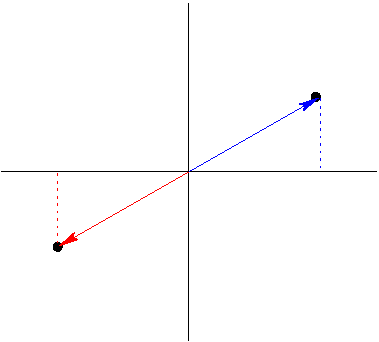
\includegraphics[scale=0.7]{figures/R2-rotate-pi.pdf}}
    % \put(2.25,0.75){\scriptsize{$0$}}
    % \put(2.05,1.6){\scriptsize{$y$}}
    % \put(3.0,0.75){\scriptsize{$x$}}
    % \put(2.85,1.22){\scriptsize{$(a,b)$}}
    % \pause
    % \put(1.0,0.5){\scriptsize{\alert{$(-a,-b)$}} }
    % \end{picture}
    \pause
    \vspace{1em}

    We see that $ R_{\pi}\left[\begin{array}{c} a \\ b \end{array}\right]
    =
    \left[\begin{array}{c} -a \\ -b \end{array}\right]
    =
    \pause\left[\begin{array}{rr} -1 & 0 \\ 0 & -1 \end{array}\right]
    \left[\begin{array}{c} a \\ b \end{array}\right],$
    so $R_{\pi}$ is a matrix transformation.
\end{example}
}
%-------------- end slide -------------------------------%}}}

%-------------- start slide -------------------------------%{{{ 34
\frame{
\begin{problem}
    The transformation $ R_{\frac{\pi}{2}}:\RR^2 \rightarrow \RR^2$
    denotes a \alert{counterclockwise} rotation about the origin
    through an angle of $\frac{\pi}{2}$ radians. Find the matrix of $R_{\frac{\pi}{2}}$.
\end{problem}
\vfill
\pause
\begin{solution}
    First,
    \[ R_{\frac{\pi}{2}}
    \left[\begin{array}{c} a \\ b \end{array}\right]
    =
    \left[\begin{array}{r} -b \\ a \end{array}\right]
    \]

    \pause
    Furthermore $R_{\frac{\pi}{2}}$ is a matrix
    transformation, and the matrix it is induced by is
    \[ \left[\begin{array}{c} -b \\ a \end{array}\right] =
    \left[\begin{array}{rr}
    0 & -1 \\ 1 & 0 \end{array}\right]
    \left[\begin{array}{c} a \\ b \end{array}\right]. \]
    \myQED
\end{solution}
}
%-------------- end slide -------------------------------%}}}

%-------------- start slide -------------------------------%{{{ 35
\frame{
\begin{example}[Rotation through $\pi/2$]
    We denote by
    \[ R_{\pi/2}:\RR^2\to\RR^2\]
    counterclockwise rotation about the origin through an angle
    of $\pi/2$.
    \pause
    \begin{center}
	    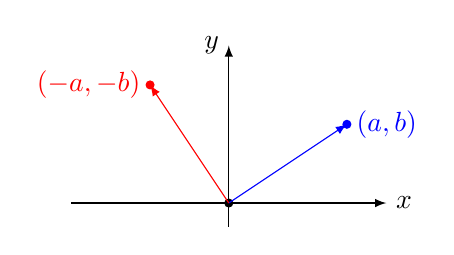
\begin{tikzpicture}[scale=1, transform shape]
	    \tikzset{>=latex}
	    \coordinate (P) at (1.5,1);
	    \coordinate (Q) at (-1,1.5);
	    \coordinate (0) at (0,0);
	    % \draw (P) -- coordinate[pos={1/3}] (A) coordinate[pos={2/3}] (B) (Q) node [right] {$Q$};
	    % \draw [->,dashed] (0) node [below] {$} -- (P) node [above] {$P$};
	    \draw [->] (-2,0) -- (2,0) node [right] {$x$};
	    \draw [->] (0,-0.3) -- (0,2) node [left] {$y$};
	    \filldraw (0) circle (0.05);
	    \pause
	    \filldraw [blue] (P) circle (0.05);
	    \draw [->,blue] (0) -- (P) node [right] {$(a,b)$};
	    \pause
	    \draw [->,red] (0) -- (Q) node [left] {\textcolor{red}{$(-a,-b)$}};
	    \filldraw[red] (Q) circle (0.05);
	    \end{tikzpicture}
    \end{center}
    \pause
    % \vspace{1em}
    % \begin{picture}(4,1.75)
    % \put(1.3,0.1){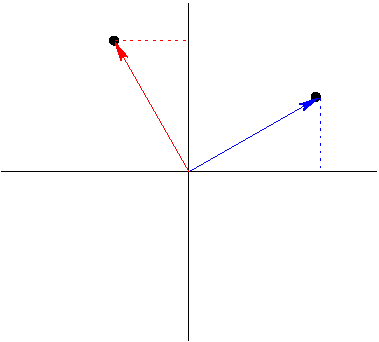
\includegraphics[scale=0.7]{figures/R2-rotate-halfpi.pdf}}
    % \put(2.25,0.75){\scriptsize{$0$}}
    % \put(2.05,1.6){\scriptsize{$y$}}
    % \put(3.0,0.75){\scriptsize{$x$}}
    % \put(2.85,1.22){\scriptsize{$(a,b)$}}
    % \pause
    % \put(1.4,1.5){\scriptsize{\alert{$(-b,a)$}} }
    % \end{picture}
    % \pause
    \pause
    We see that $ R_{\pi/2}\left[\begin{array}{c} a \\ b \end{array}\right]
    =
    \left[\begin{array}{c} -b \\ a \end{array}\right]
    =
    \pause\left[\begin{array}{rr} 0 & -1 \\ 1 & 0 \end{array}\right]
    \left[\begin{array}{c} a \\ b \end{array}\right],$
    so $R_{\pi/2}$ is a matrix transformation.
    \end{example}
}
%-------------- end slide -------------------------------%}}}

%-------------- start slide -------------------------------%{{{ 36
\frame{
\frametitle{Reflection in $\RR^2$}
\pause
\begin{example}
    In $\RR^2$, reflection in the $x$-axis, which transforms
    $\left[\begin{array}{r} a \\ b \end{array}\right]$ to
    $\left[\begin{array}{r} a \\ -b \end{array}\right]$,
    is a matrix transformation because
    \[ \left[\begin{array}{r} a \\ -b \end{array}\right] =
    \left[ \begin{array}{rr}
    1 & 0 \\ 0 & -1 \end{array}\right]
    \left[\begin{array}{r} a \\ b \end{array}\right].\]
\end{example}
\pause
\vfill
\begin{example}
    In $\RR^2$, reflection in the $y$-axis transforms
    $\left[\begin{array}{r} a \\ b \end{array}\right]$ to
    $\left[\begin{array}{r} -a \\ b \end{array}\right]$.
    This is a matrix transformation because
    \[ \left[\begin{array}{r} -a \\ b \end{array}\right] =
    \left[ \begin{array}{rr}
    -1 & 0 \\ 0 & 1 \end{array}\right]
    \left[\begin{array}{r} a \\ b \end{array}\right].\]
\end{example}
}
%-------------- end slide -------------------------------%}}}

%-------------- start slide -------------------------------%{{{ 37
\frame{
\begin{example}
    Reflection in the line $y=x$
    transforms
    $\left[\begin{array}{r} a \\ b \end{array}\right]$ to
    $\left[\begin{array}{r} b \\ a \end{array}\right]$.
    \vspace{1em}
    \pause
    \begin{center}
	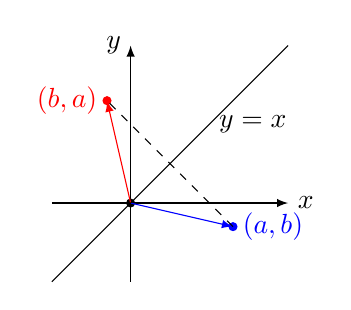
\begin{tikzpicture}[scale=1, transform shape]
	    \tikzset{>=latex}
	    \coordinate (P) at (1.3,-0.3);
	    \coordinate (Q) at (-0.3,1.3);
	    \coordinate (0) at (0,0);
	    \draw [->] (-1,0) -- (2,0) node [right] {$x$};
	    \draw [->] (0,-1) -- (0,2) node [left] {$y$};
	    \filldraw (0) circle (0.05);
	    \filldraw [blue] (P) circle (0.05);
	    \draw [->,blue] (0) -- (P) node [right] {$(a,b)$};
	    \draw [->,red] (0) -- (Q) node [left] {\textcolor{red}{$(b,a)$}};
	    \filldraw[red] (Q) circle (0.05);
	    \draw (-1,-1) -- (1,1) node [right] {$y=x$} -- (2,2);
	    \draw [dashed] (P) -- (Q);
	\end{tikzpicture}
    \end{center}

    % \begin{picture}(4,1.5)
    % \put(1.4,0){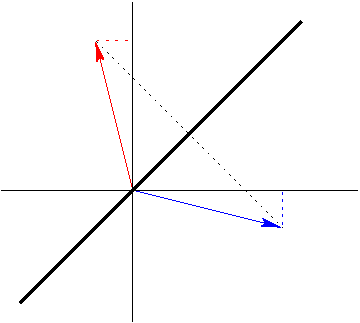
\includegraphics[scale=0.75]{figures/eigenvectors-2.pdf}}
    % \put(2.85,0.45){\textcolor{blue}{{\scriptsize{$(a,b)$}} }}
    % \put(1.55,1.4){\textcolor{red}{{\scriptsize{$(b,a)$}} }}
    % \put(3.2,0.63){\scriptsize{$x$}}
    % \put(2.1,1.5){\scriptsize{$y$}}
    % \put(2.8,1.3){\scriptsize{$y=x$}}
    % \end{picture}
    \pause
    \vspace{1em}

    This is a matrix transformation because
    \[ \left[\begin{array}{r} b \\ a \end{array}\right] =
    \left[ \begin{array}{rr}
    0 & 1 \\ 1 & 0 \end{array}\right]
    \left[\begin{array}{r} a \\ b \end{array}\right].\]
\end{example}
}
%-------------- end slide -------------------------------%}}}

%-------------- start slide -------------------------------%{{{ 38
\frame{
\frametitle{Reflection in the line}
\pause
\begin{example}[ Reflection in $y=mx$ preserves scalar multiplication ]
    % \textcolor{titletextcolour}{Example (Reflection in $y=mx$ preserves scalar multiplication)}\\[0.5em]
    Let $Q_m:\RR^2\rightarrow \RR^2$ denote reflection in the
    line $y=mx$, and let $\vec{u}\in\RR^2$.
    \vspace{1em}
    \pause

    \begin{picture}(4,1.5)
	\uncover<2>{
	    \put(0.3,0){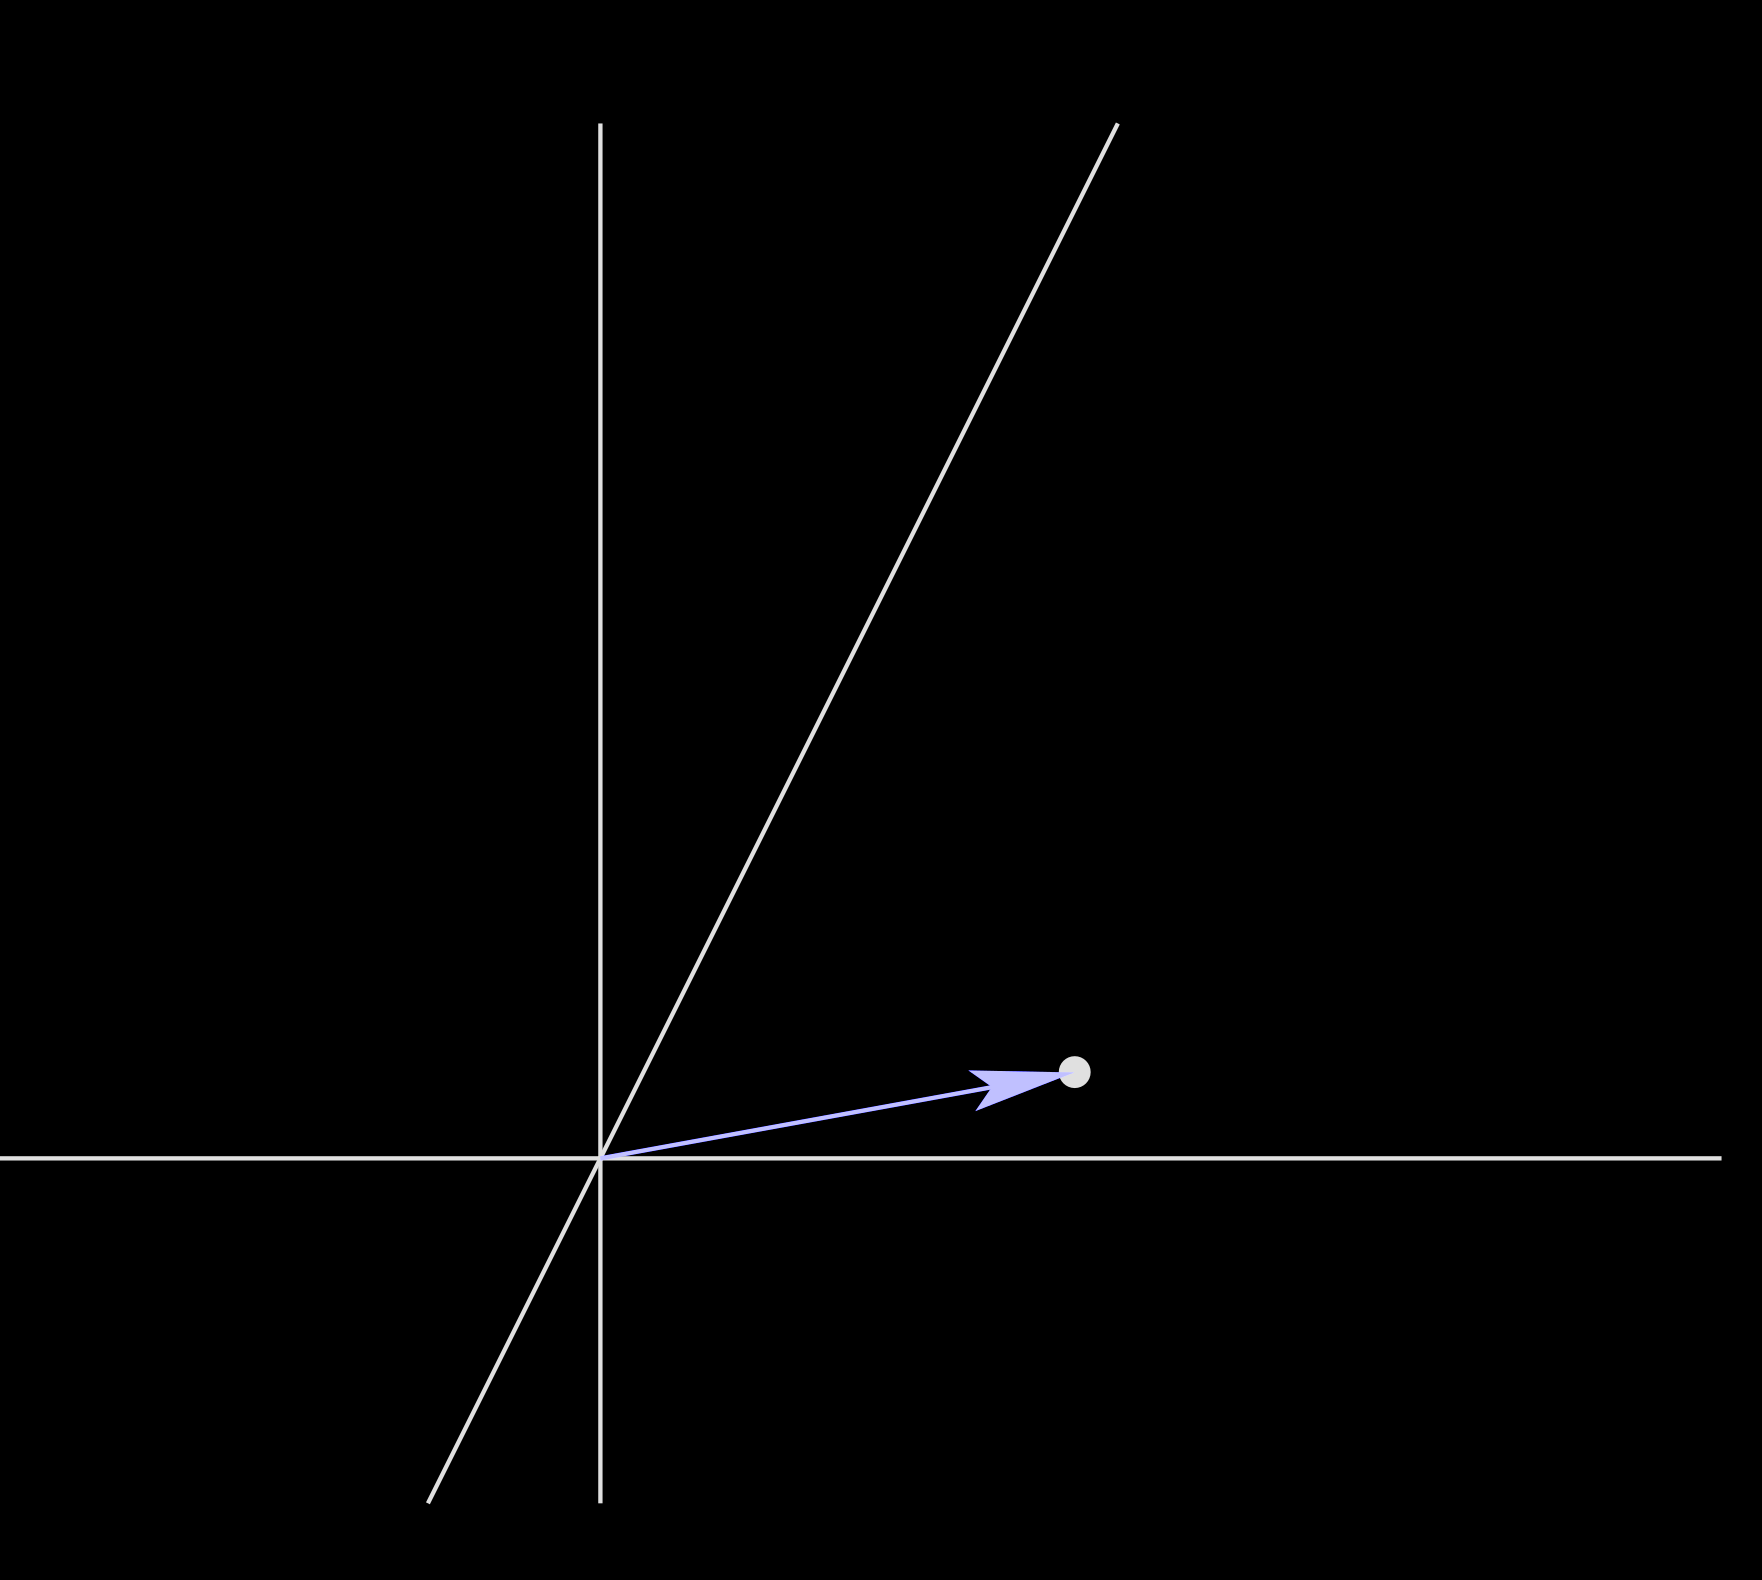
\includegraphics[scale=0.07]{figures/vectors-23a_copy.png}}
	    \put(1.45,1.25){\scriptsize{$y=mx$}}
	    \put(0.95,1.25){\scriptsize{$y$}}
	    \put(1.95,0.25){\scriptsize{$x$}}
	    \put(1.15,0.45){\scriptsize{\textcolor{blue}{$\vec{u}$}} }
	}
	\uncover<3-5>{
	    \put(0.3,0){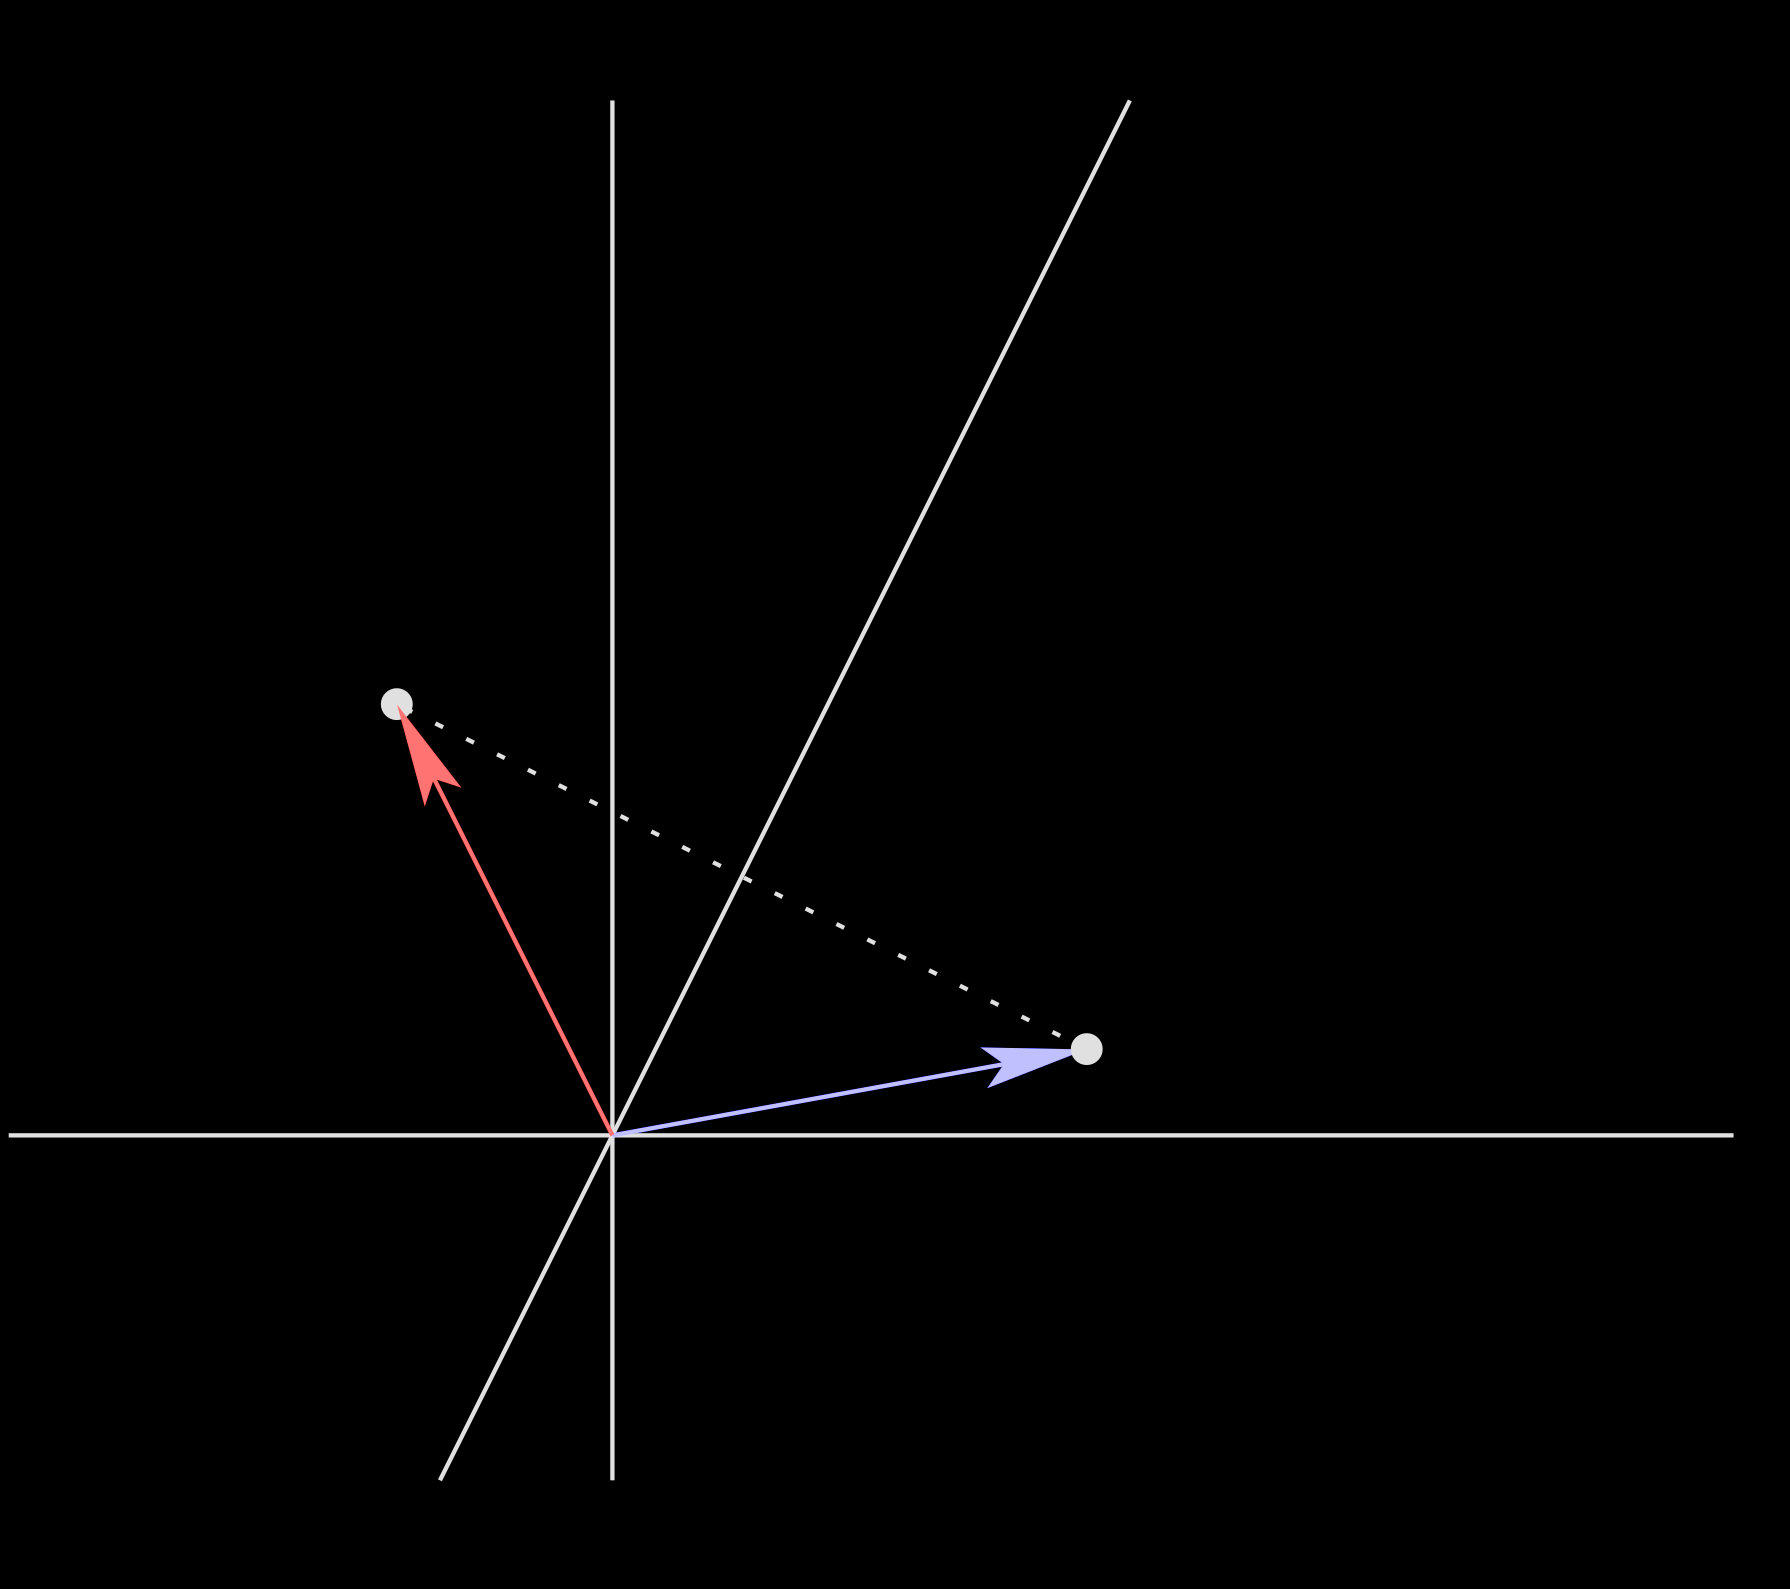
\includegraphics[scale=0.07]{figures/vectors-23b_copy.png}}
	    \put(1.45,1.25){\scriptsize{$y=mx$}}
	    \put(0.95,1.25){\scriptsize{$y$}}
	    \put(1.95,0.25){\scriptsize{$x$}}
	    \put(1.15,0.45){\scriptsize{\textcolor{blue}{$\vec{u}$}} }
	    \put(0.4,0.55){\scriptsize{\textcolor{red}{$Q_m(\vec{u})$}} }
	}
	\uncover<4>{
	    \put(2.5,0){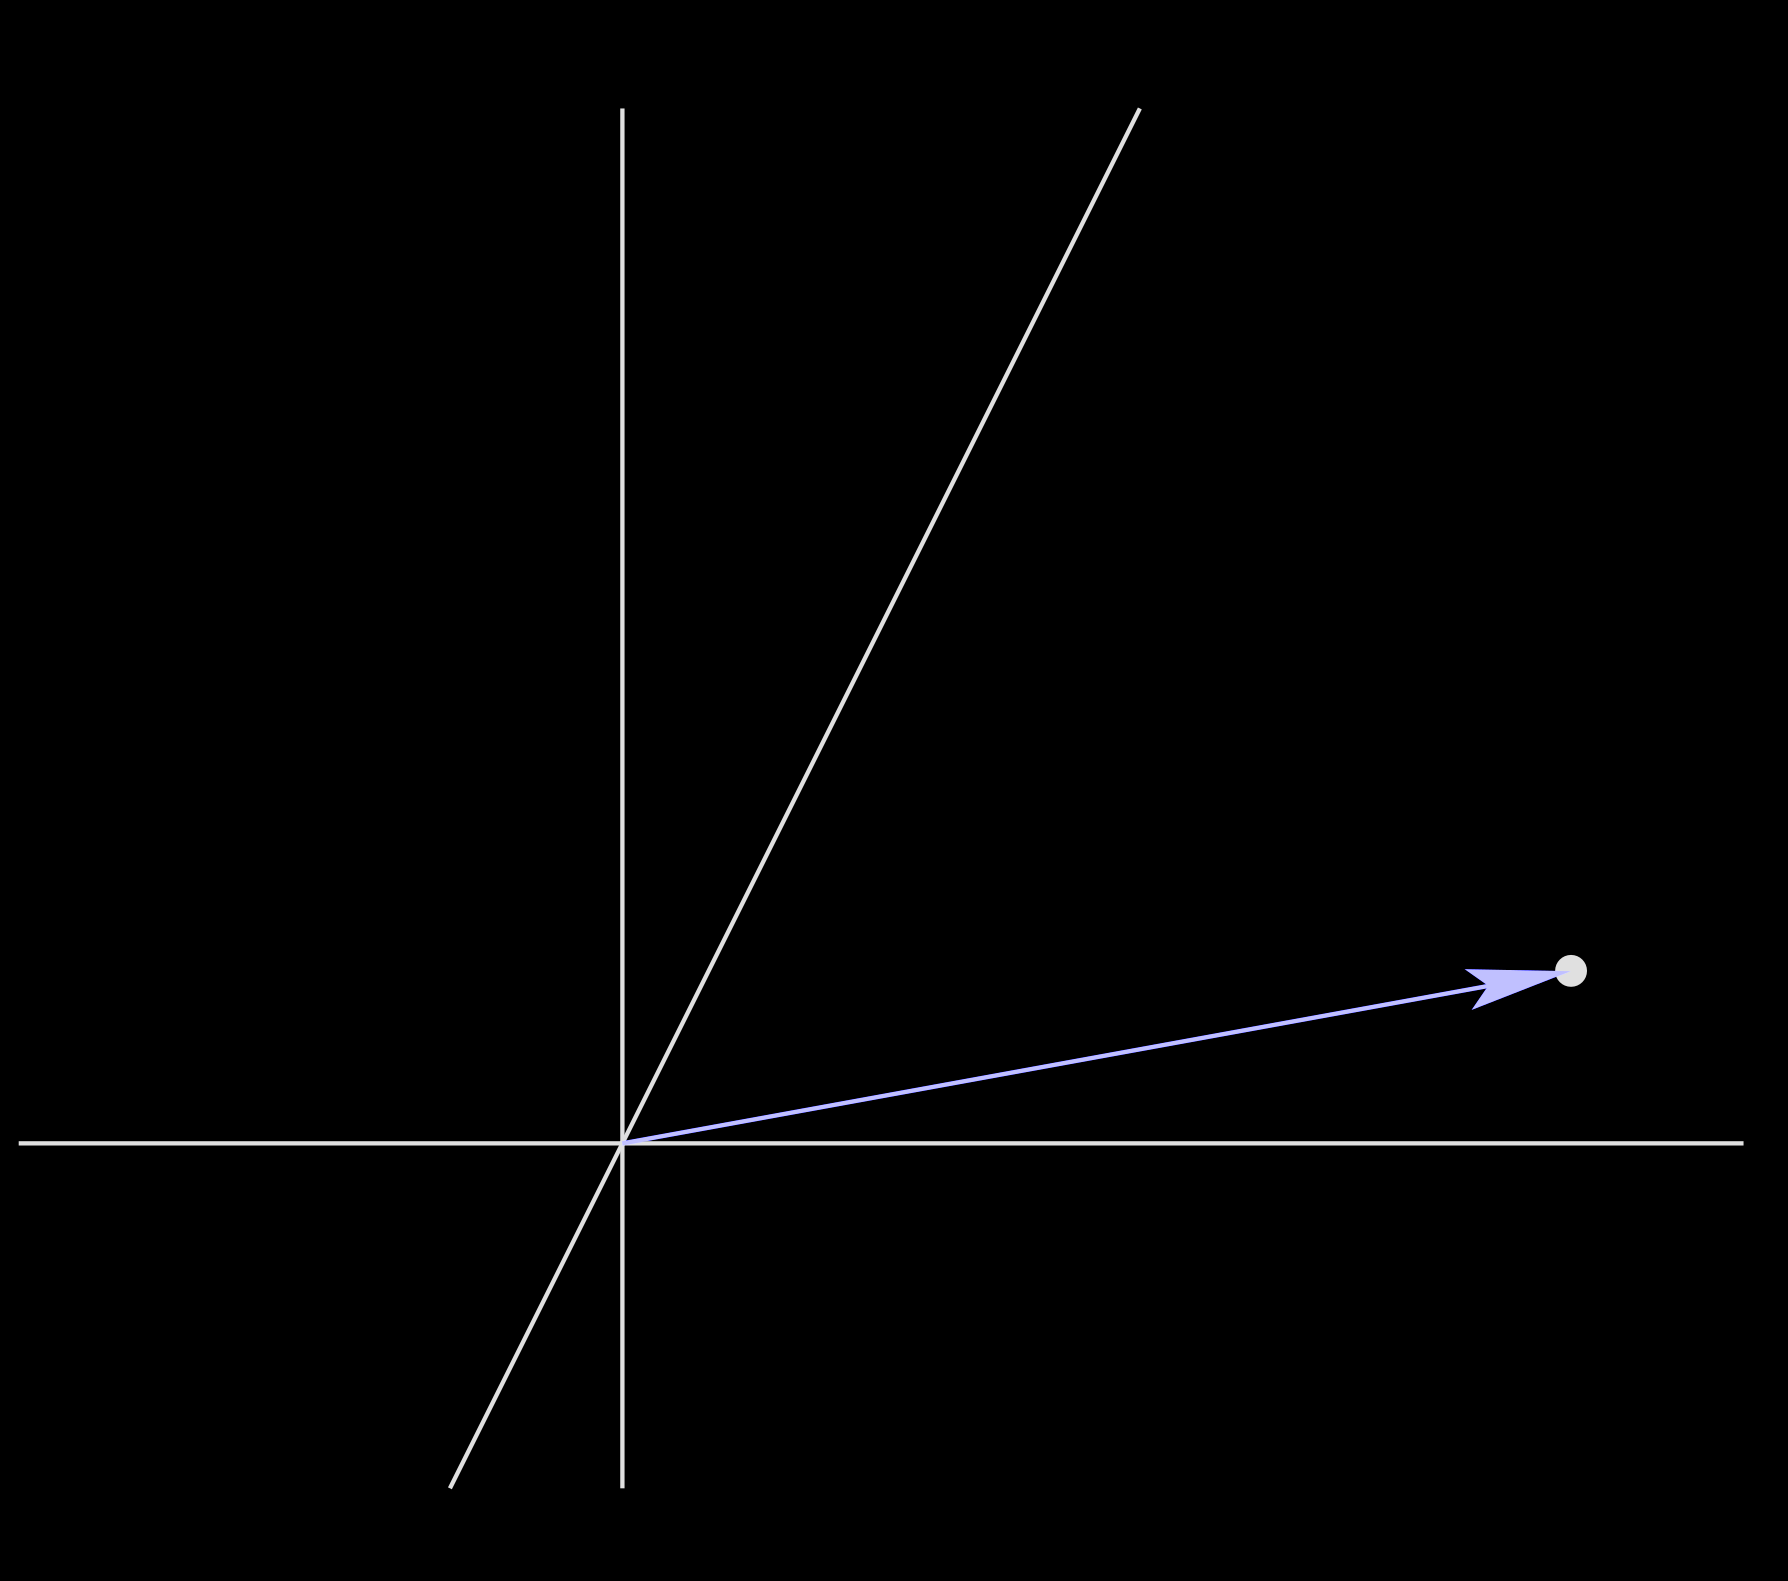
\includegraphics[scale=0.07]{figures/vectors-24a_copy.png}}
	}
	\uncover<4->{
	    \put(3.15,1.25){\scriptsize{$y$}}
	    \put(4.15,0.25){\scriptsize{$x$}}
	    \put(3.65,1.25){\scriptsize{$y=mx$}}
	    \put(3.5,0.5){\scriptsize{\textcolor{blue}{$2\vec{u}$}} }
	}
	\uncover<5->{
	    \put(2.5,0){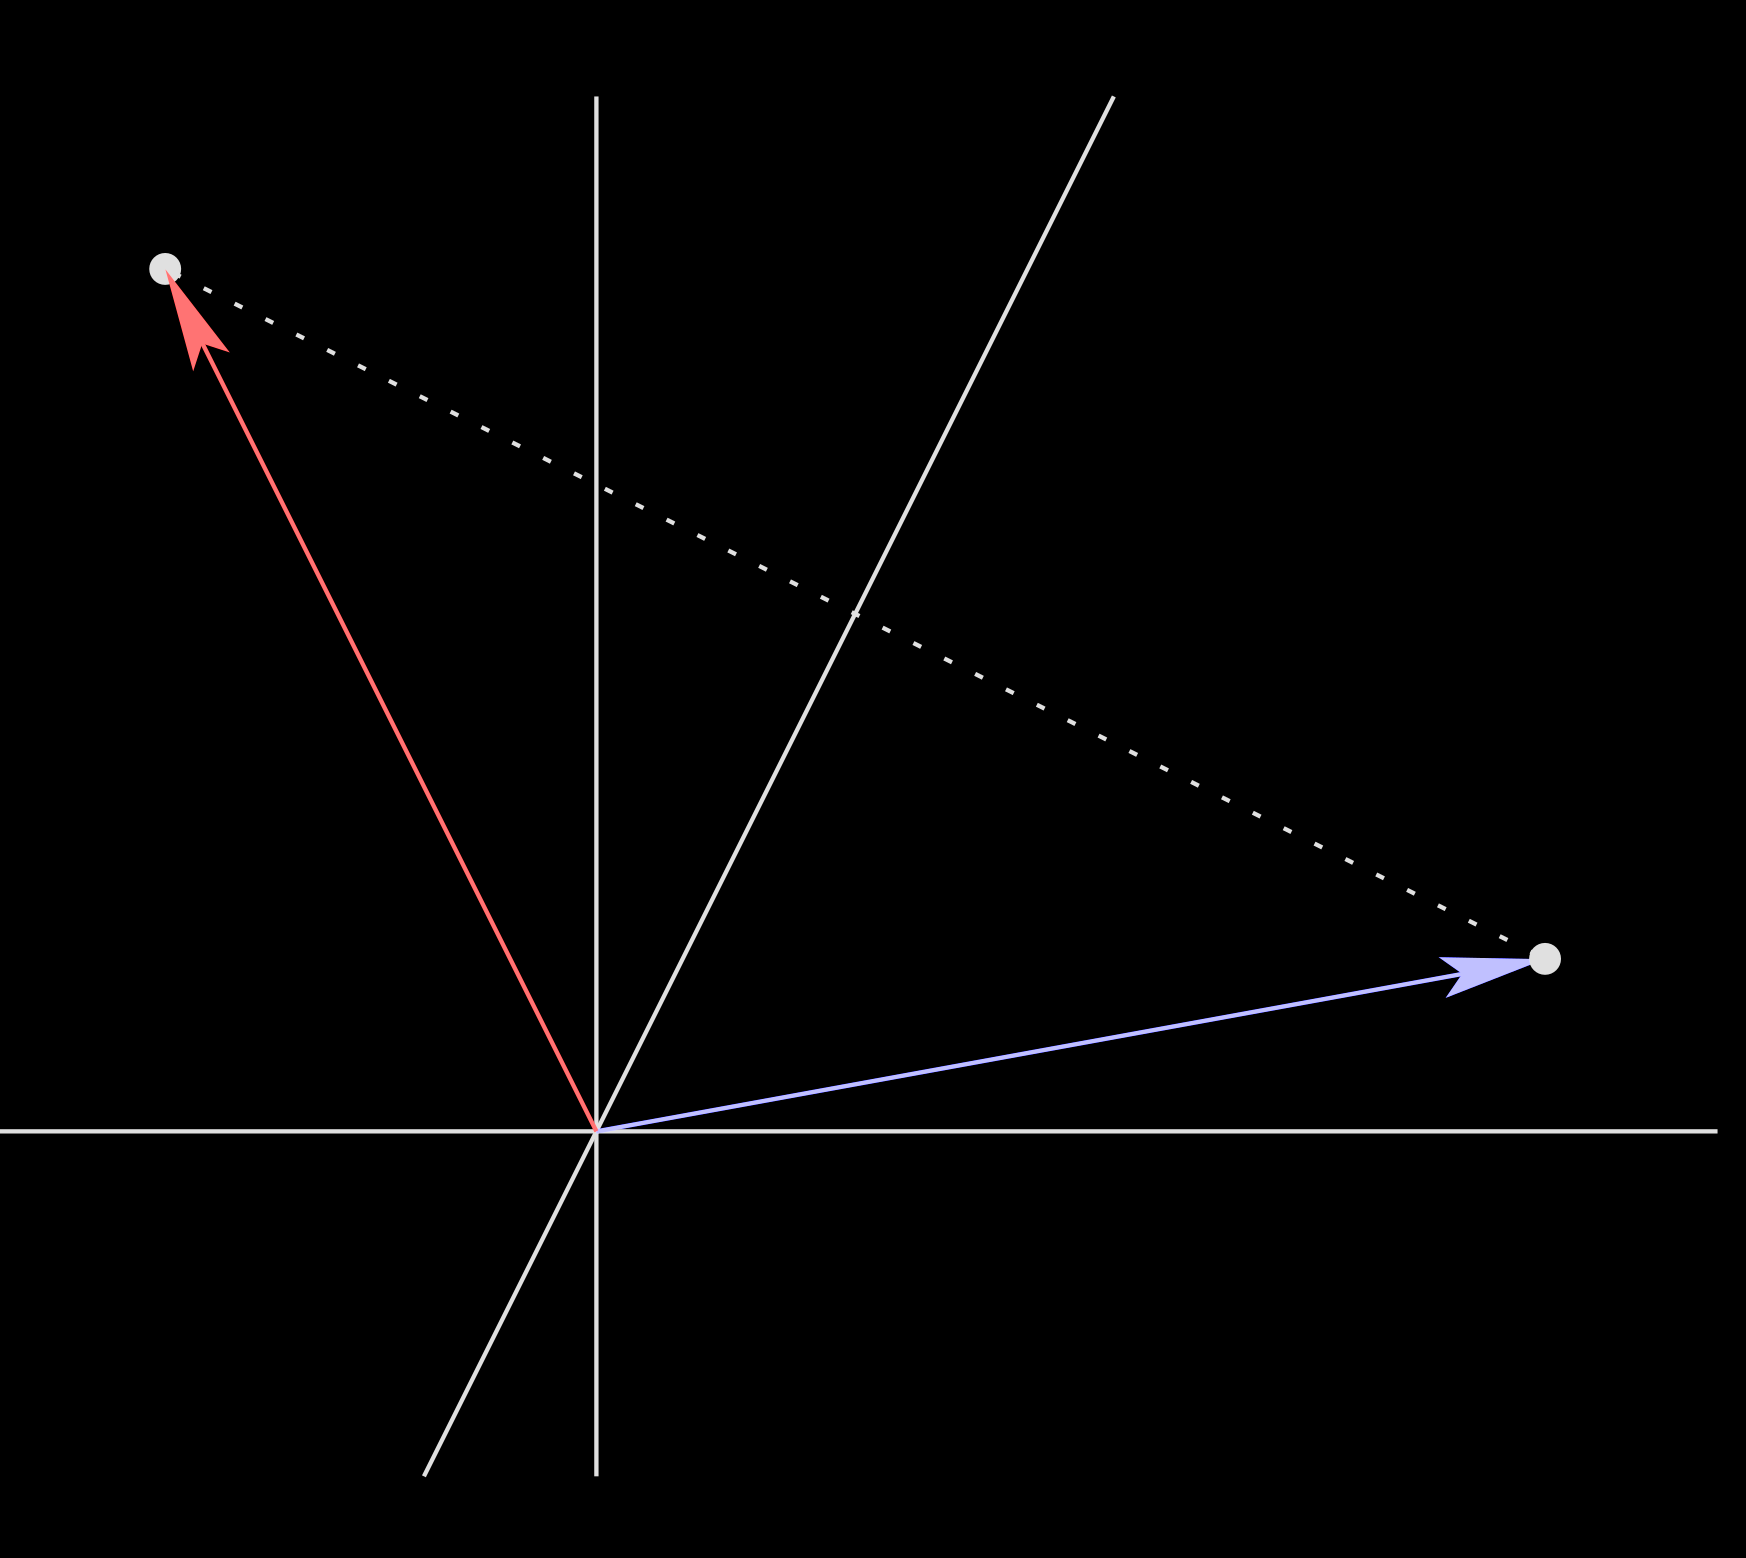
\includegraphics[scale=0.07]{figures/vectors-24_copy.png}}
	    \put(3.15,1.25){\scriptsize{$y$}}
	    \put(4.15,0.25){\scriptsize{$x$}}
	    \put(3.65,1.25){\scriptsize{$y=mx$}}
	    \put(3.5,0.5){\scriptsize{\textcolor{blue}{$2\vec{u}$}} }
	    \put(2.45,0.8){\scriptsize{\textcolor{red}{$Q_m(2\vec{u})$}} }
	}
	\uncover<6->{
	    \put(0.3,0){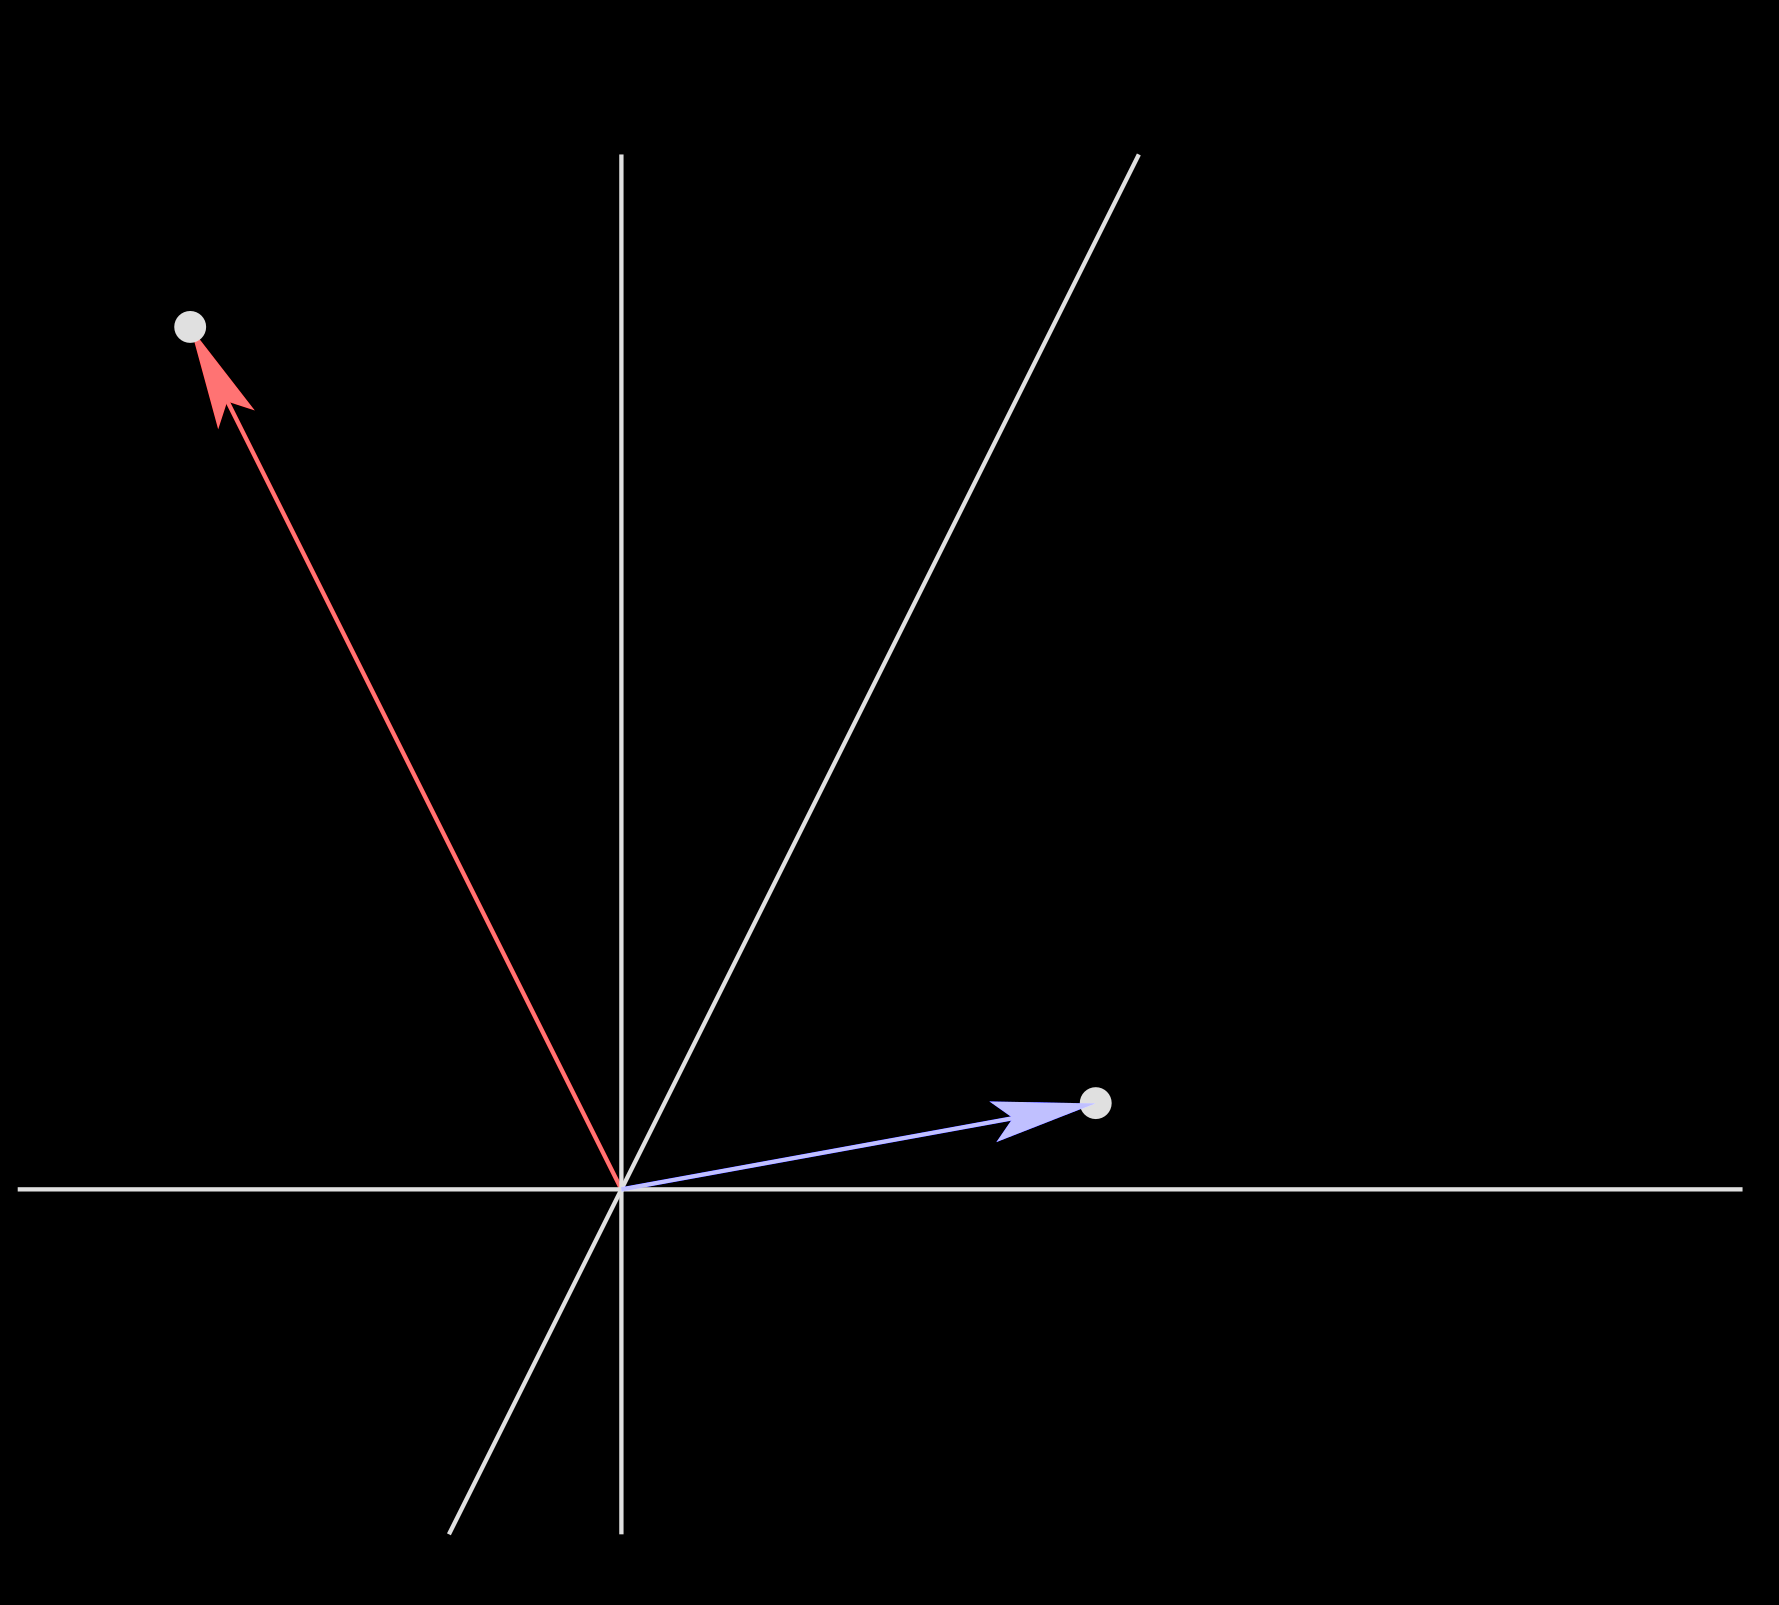
\includegraphics[scale=0.07]{figures/vectors-23_copy.png}}
	    \put(0.2,0.9){\scriptsize{\textcolor{red}{$2Q_m(\vec{u})$}} }
	    \put(2.45,0.8){\scriptsize{\textcolor{red}{$Q_m(2\vec{u})$}} }
	}
    \end{picture}
    \bigskip

    \uncover<6->{
	The figure indicates that \alert{$Q_m(2\vec{u})=2Q_m(\vec{u})$.}
    }
    \uncover<7->{
	In general, for any scalar $k$,
	\[ Q_m(kX)=kQ_m(X), \]
    }
    \uncover<8->{
	i.e., $Q_m$ preserves scalar multiplication.
    }
\end{example}
}
%-------------- end slide -------------------------------%}}}

%-------------- start slide -------------------------------%{{{ 39
\frame{
    \begin{example}[ Reflection in $y=mx$ preserves vector addition ]
    % \textcolor{titletextcolour}{Example (Reflection in $y=mx$ preserves vector addition)}\\[0.5em]
    Let $\vec{u},\vec{v}\in\RR^2$.

    \begin{picture}(4,1.5)
	\uncover<2>{
	\put(0.3,0){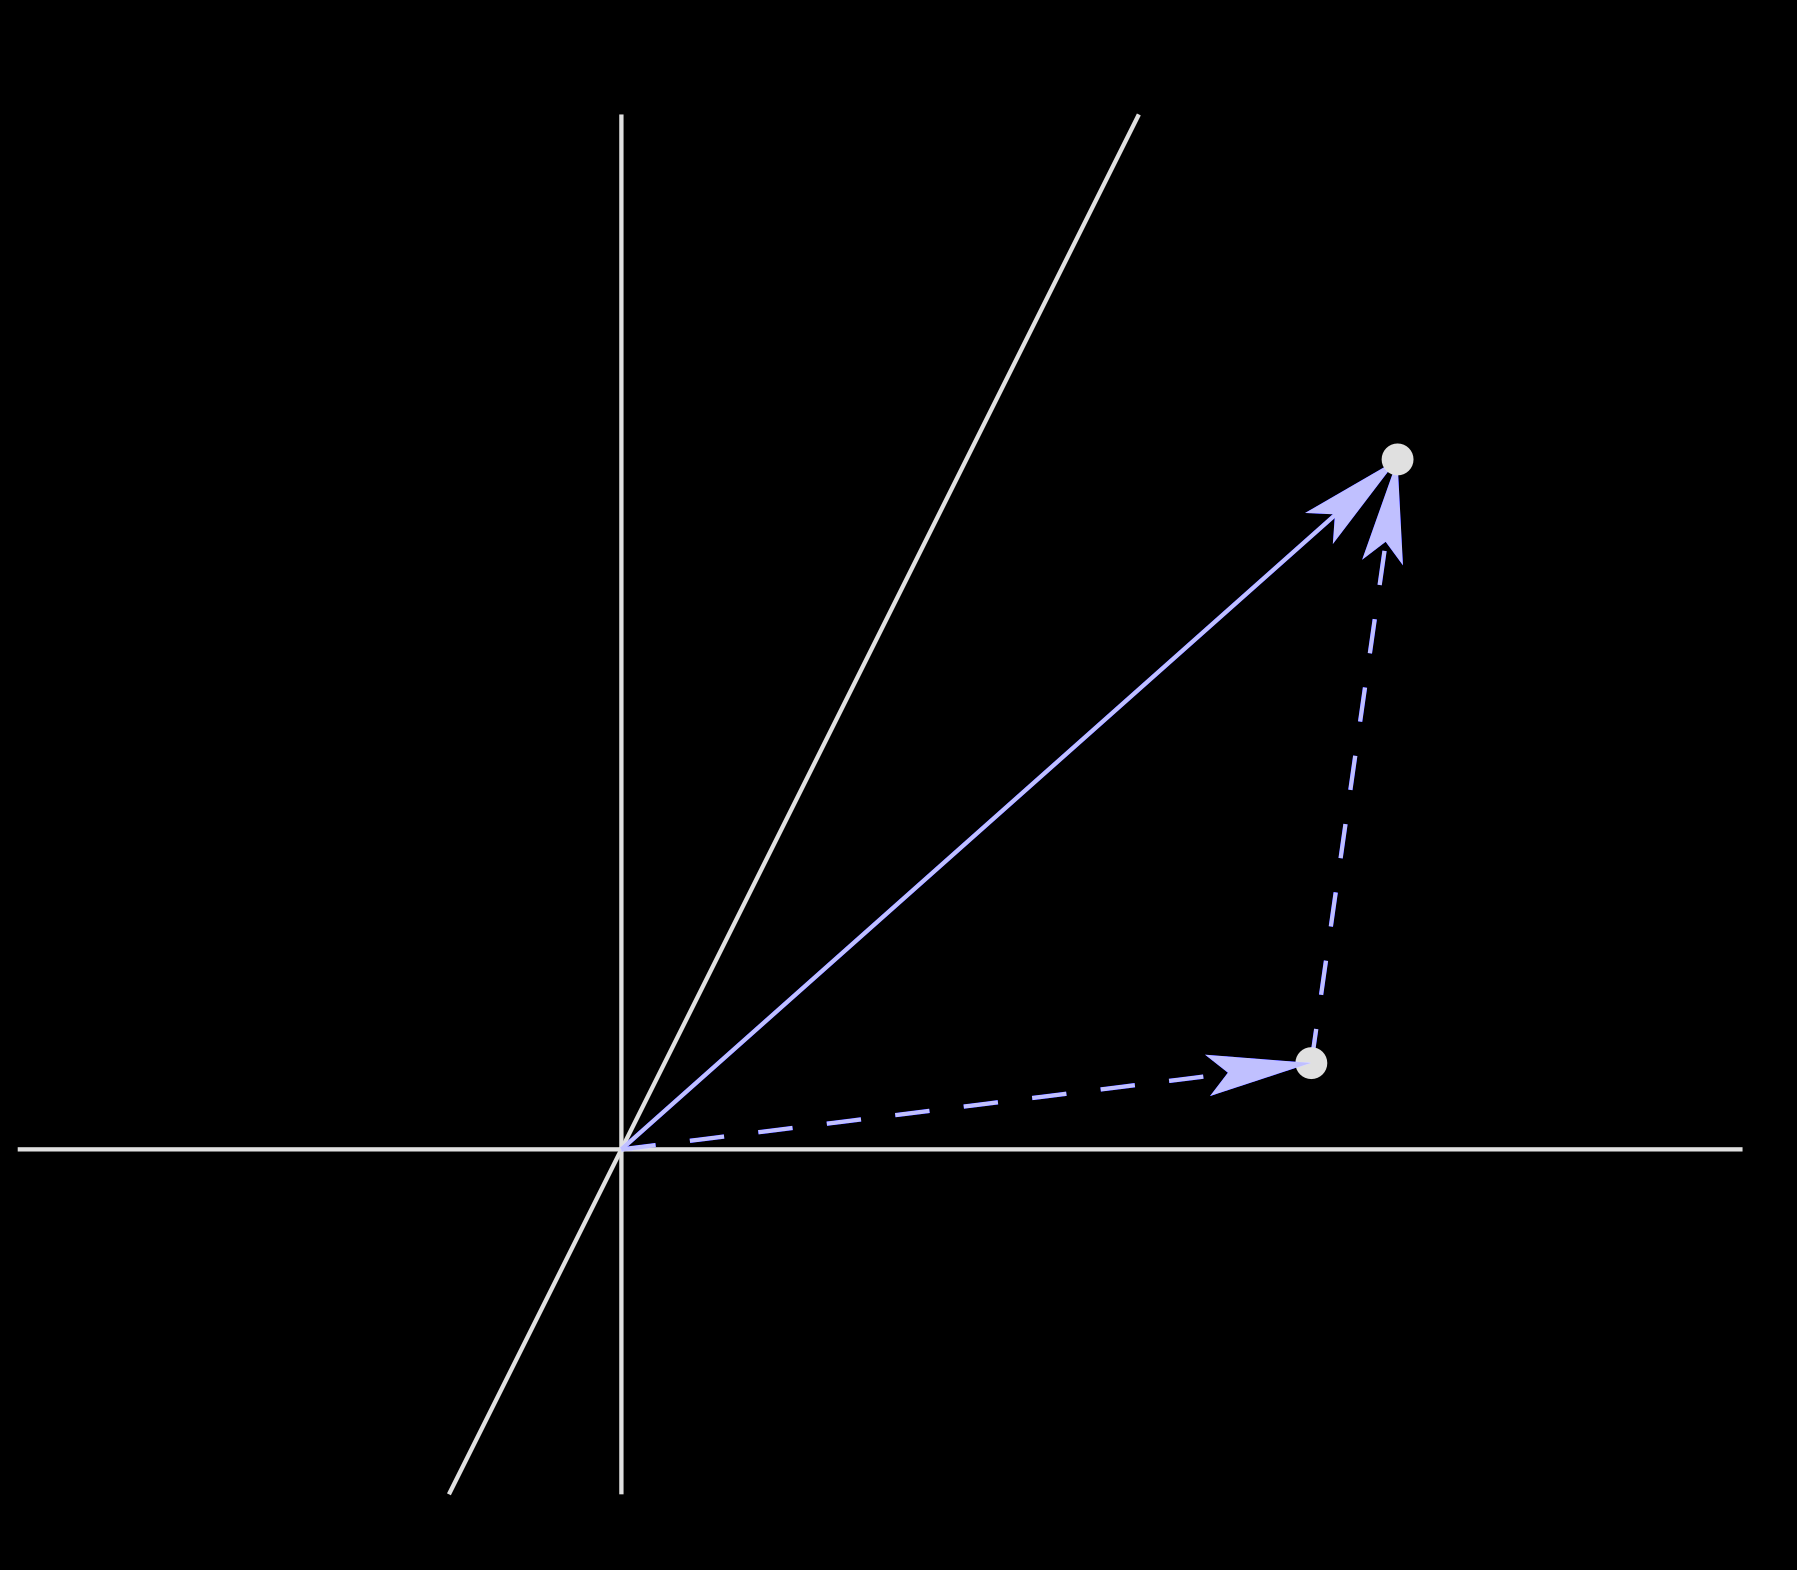
\includegraphics[scale=0.07]{figures/vectors-25a_copy.png}} }
	\uncover<2->{
	    \put(1.45,1.25){\scriptsize{$y=mx$}}
	    \put(0.8,1.25){\scriptsize{$y$}}
	    \put(1.95,0.25){\scriptsize{$x$}}
	    \put(1.25,0.47){\scriptsize{\textcolor{blue}{$\vec{u}$}} }
	    \put(1.7,0.7){\scriptsize{\textcolor{blue}{$\vec{v}$}} }
	    \put(1.2,0.85){\scriptsize{\textcolor{blue}{$\vec{u}+\vec{v}$}} }
	}
	\uncover<3->{
	    \put(0.3,0){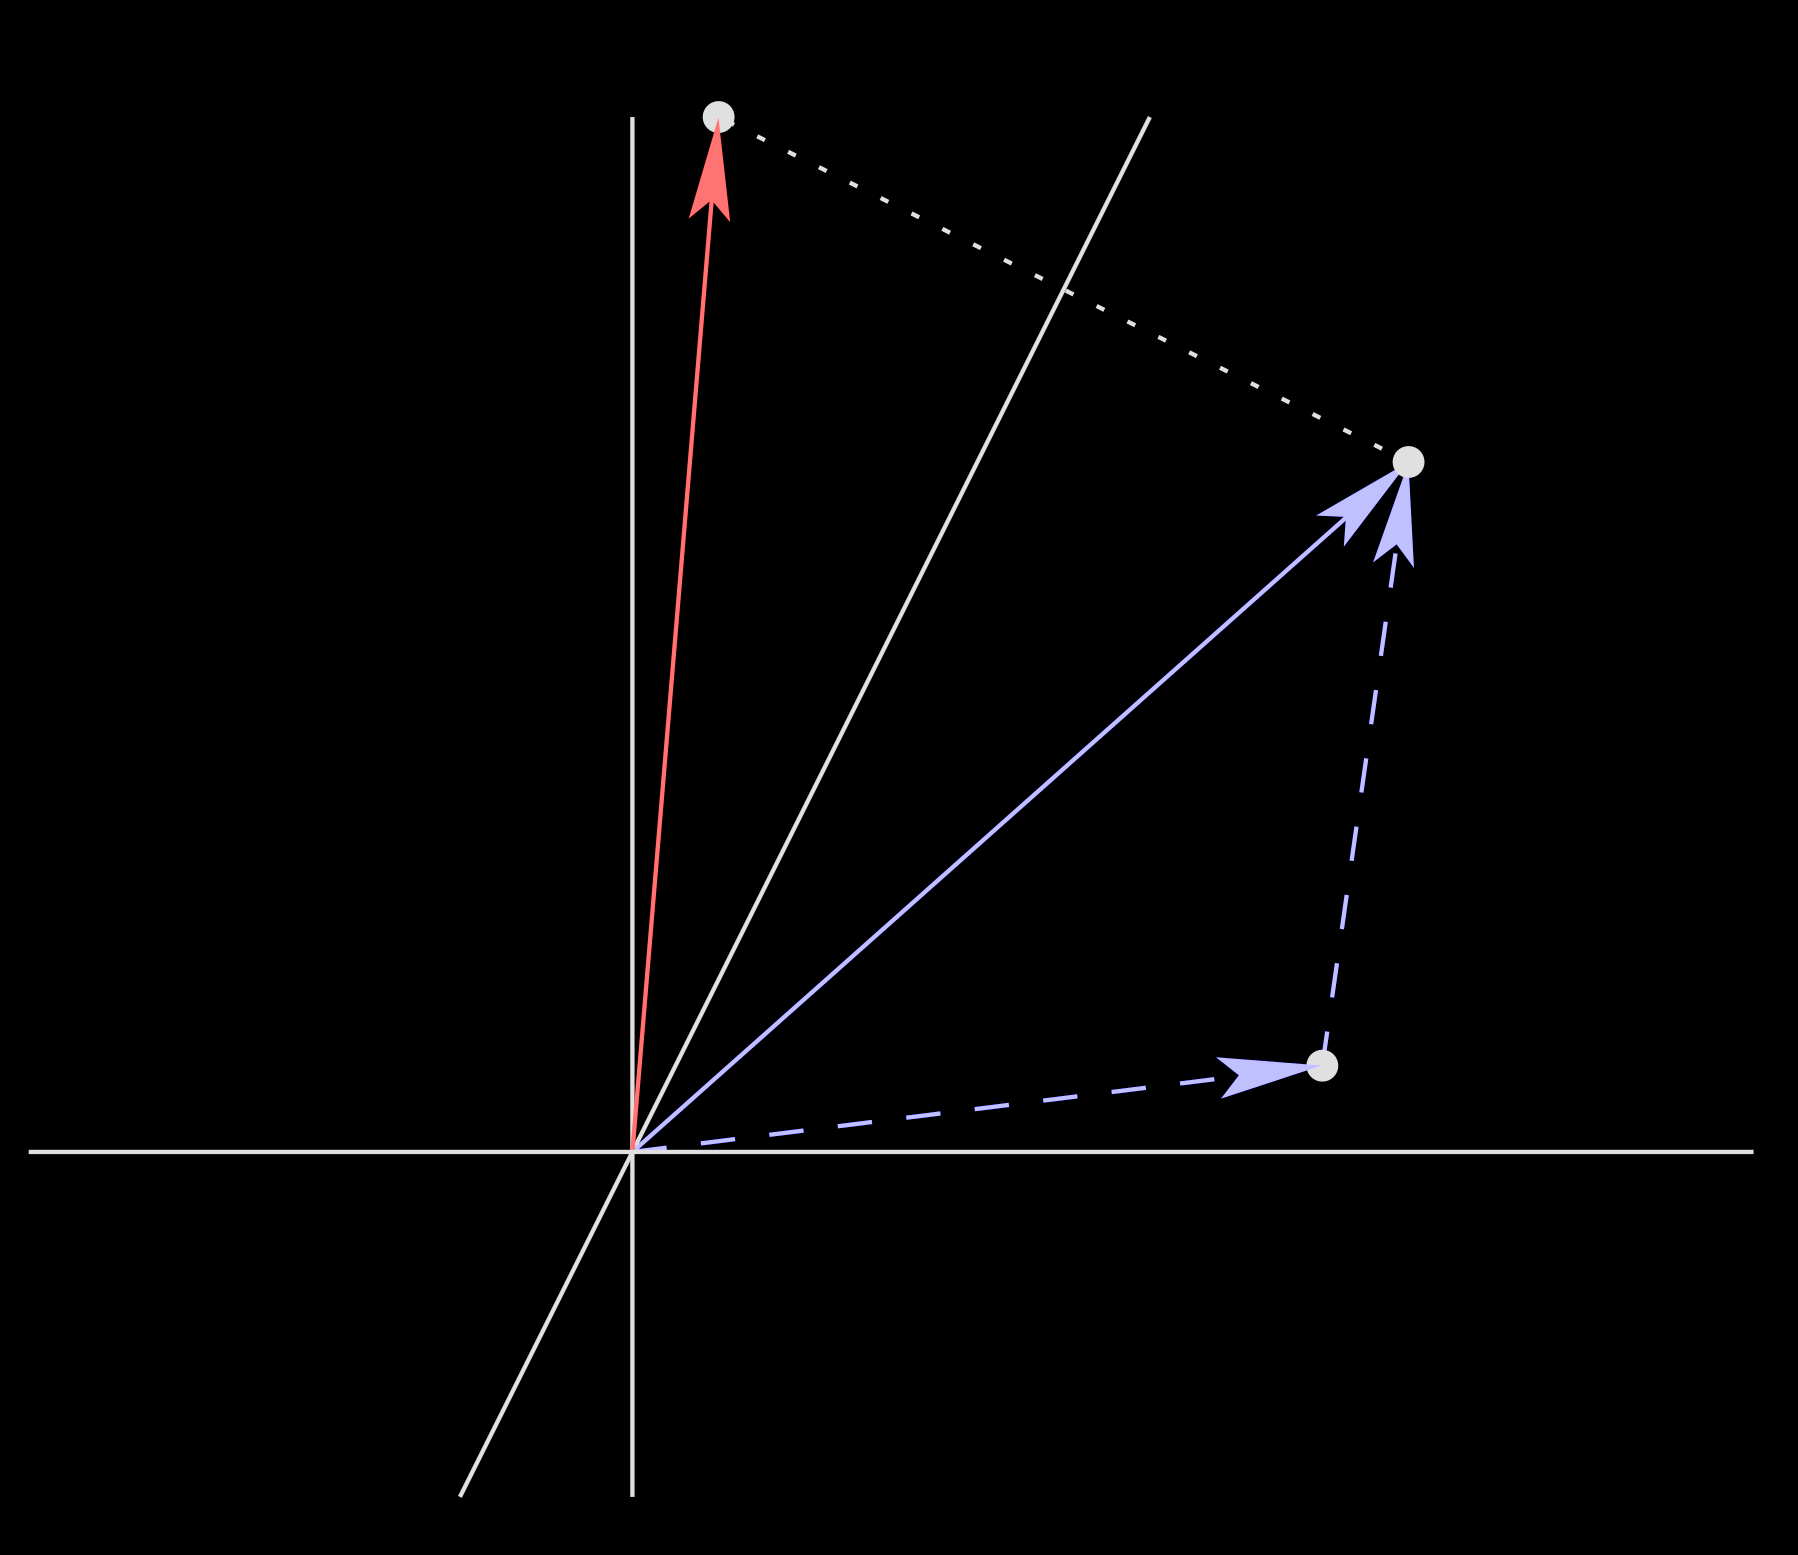
\includegraphics[scale=0.07]{figures/vectors-25_copy.png}}
	    \put(0.35,0.85){\scriptsize{\textcolor{red}{$Q_m(\vec{u}+\vec{v})$}} }
	    \put(1.45,1.25){\scriptsize{$y=mx$}}
	    \put(0.8,1.25){\scriptsize{$y$}}
	    \put(1.95,0.25){\scriptsize{$x$}}
	    \put(1.25,0.47){\scriptsize{\textcolor{blue}{$\vec{u}$}} }
	    \put(1.7,0.7){\scriptsize{\textcolor{blue}{$\vec{v}$}} }
	    \put(1.2,0.85){\scriptsize{\textcolor{blue}{$\vec{u}+\vec{v}$}} }
	}
	\uncover<4>{
	\put(2.5,0){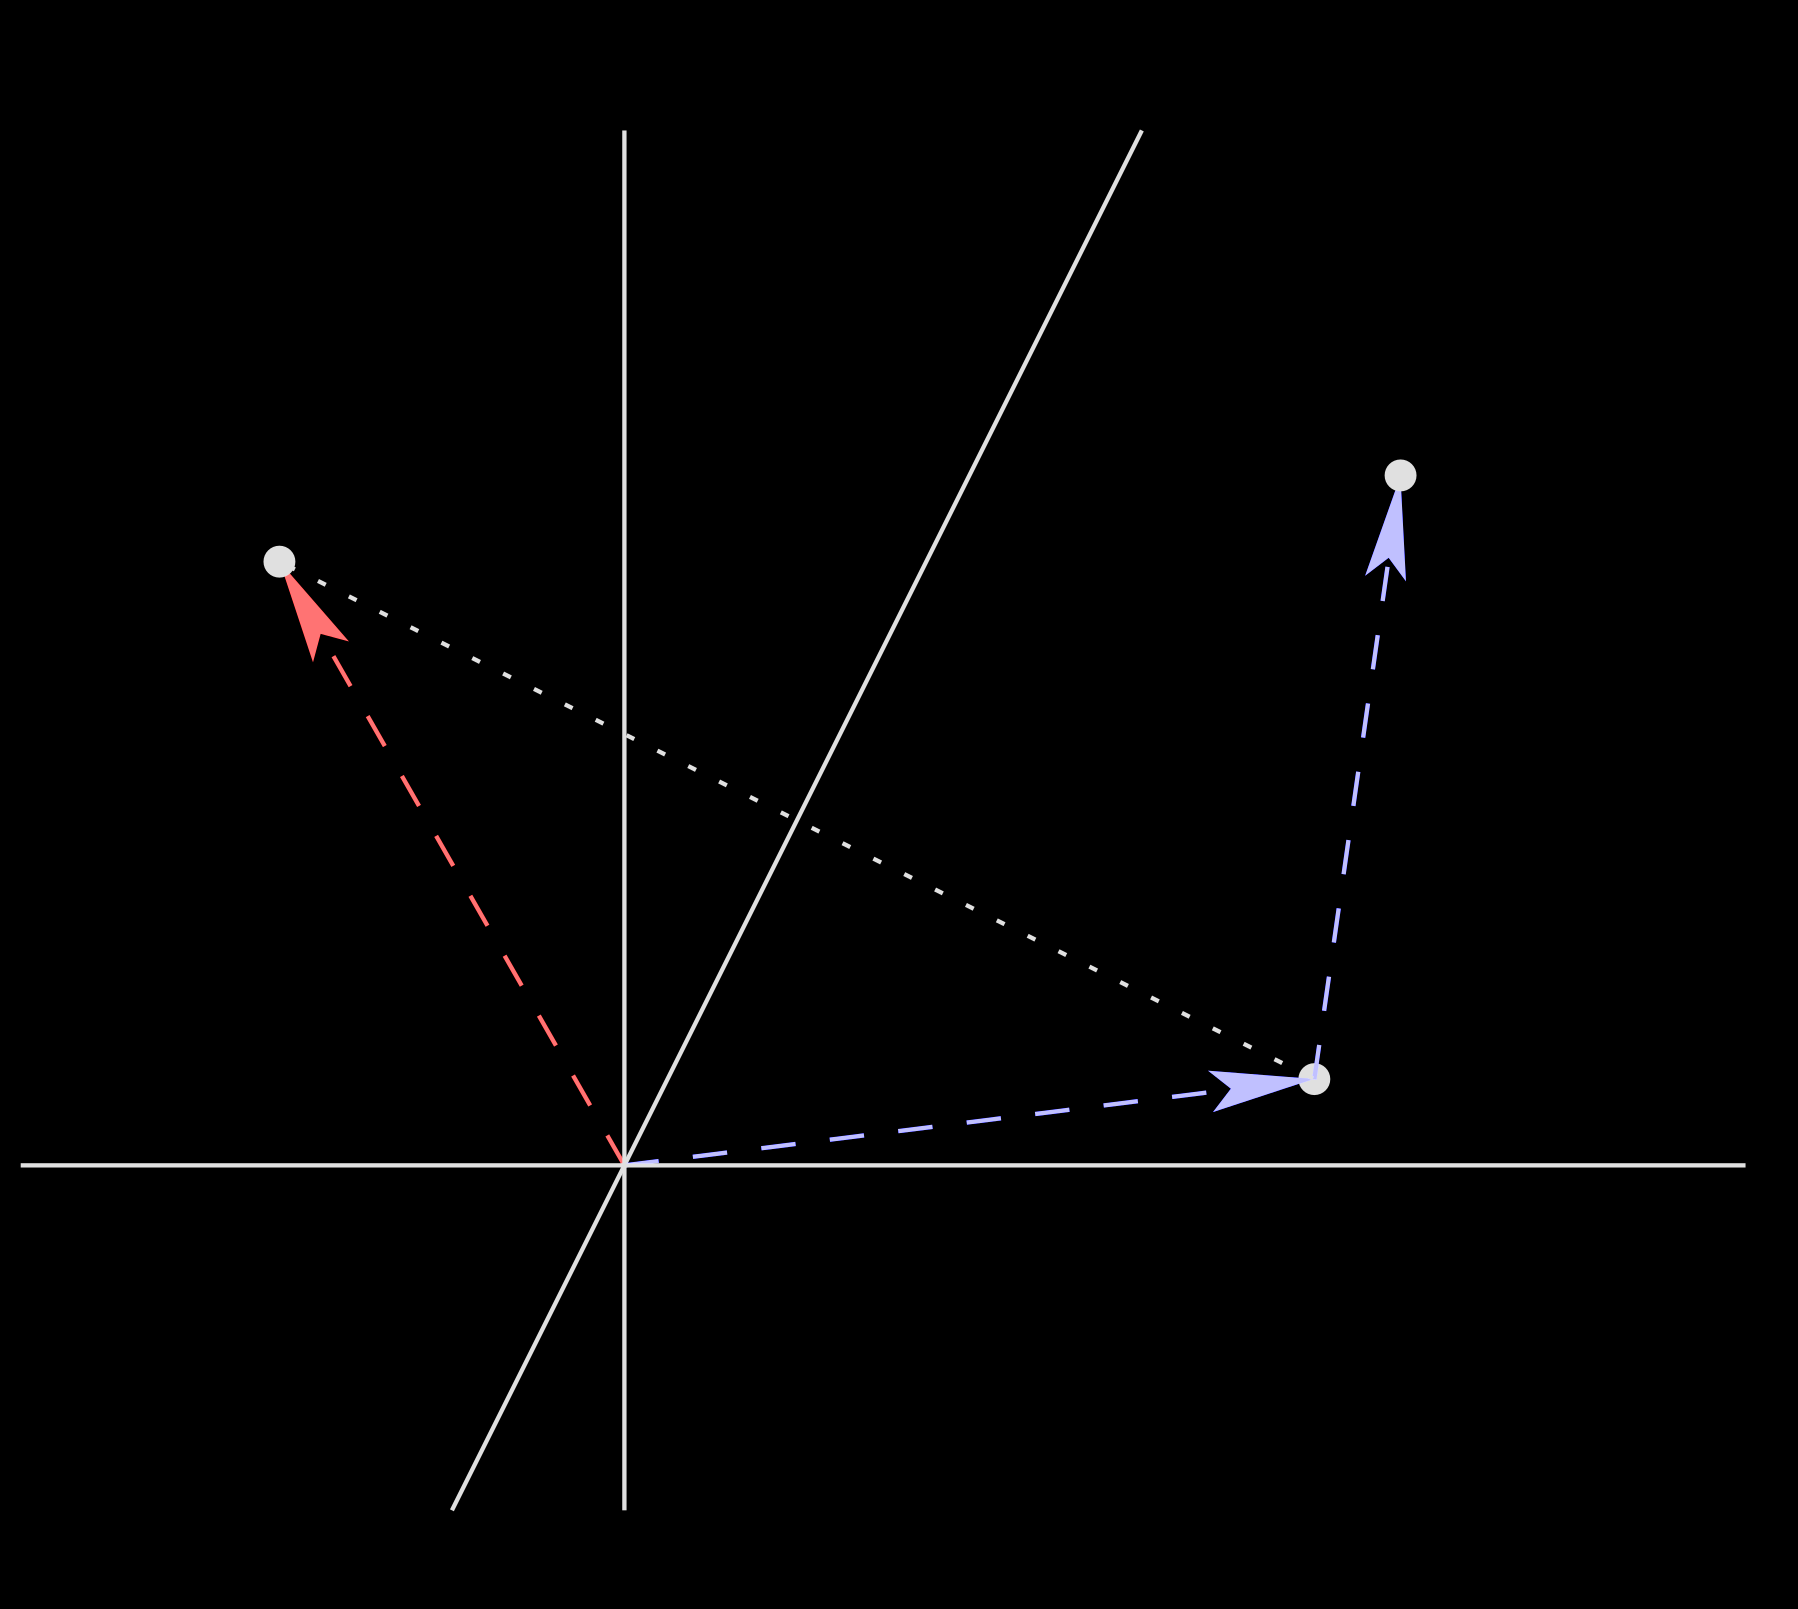
\includegraphics[scale=0.07]{figures/vectors-26a_copy.png}} }
	\uncover<4->{
	    \put(3.65,1.25){\scriptsize{$y=mx$}}
	    \put(3.0,1.35){\scriptsize{$y$}}
	    \put(4.15,0.25){\scriptsize{$x$}}
	    \put(3.4,0.45){\scriptsize{\textcolor{blue}{$\vec{u}$}} }
	    \put(3.9,0.7){\scriptsize{\textcolor{blue}{$\vec{v}$}} }
	    \put(2.6,0.6){\scriptsize{\textcolor{red}{$Q_m(\vec{u})$}} }
	}
	\uncover<5>{
	    \put(2.5,0){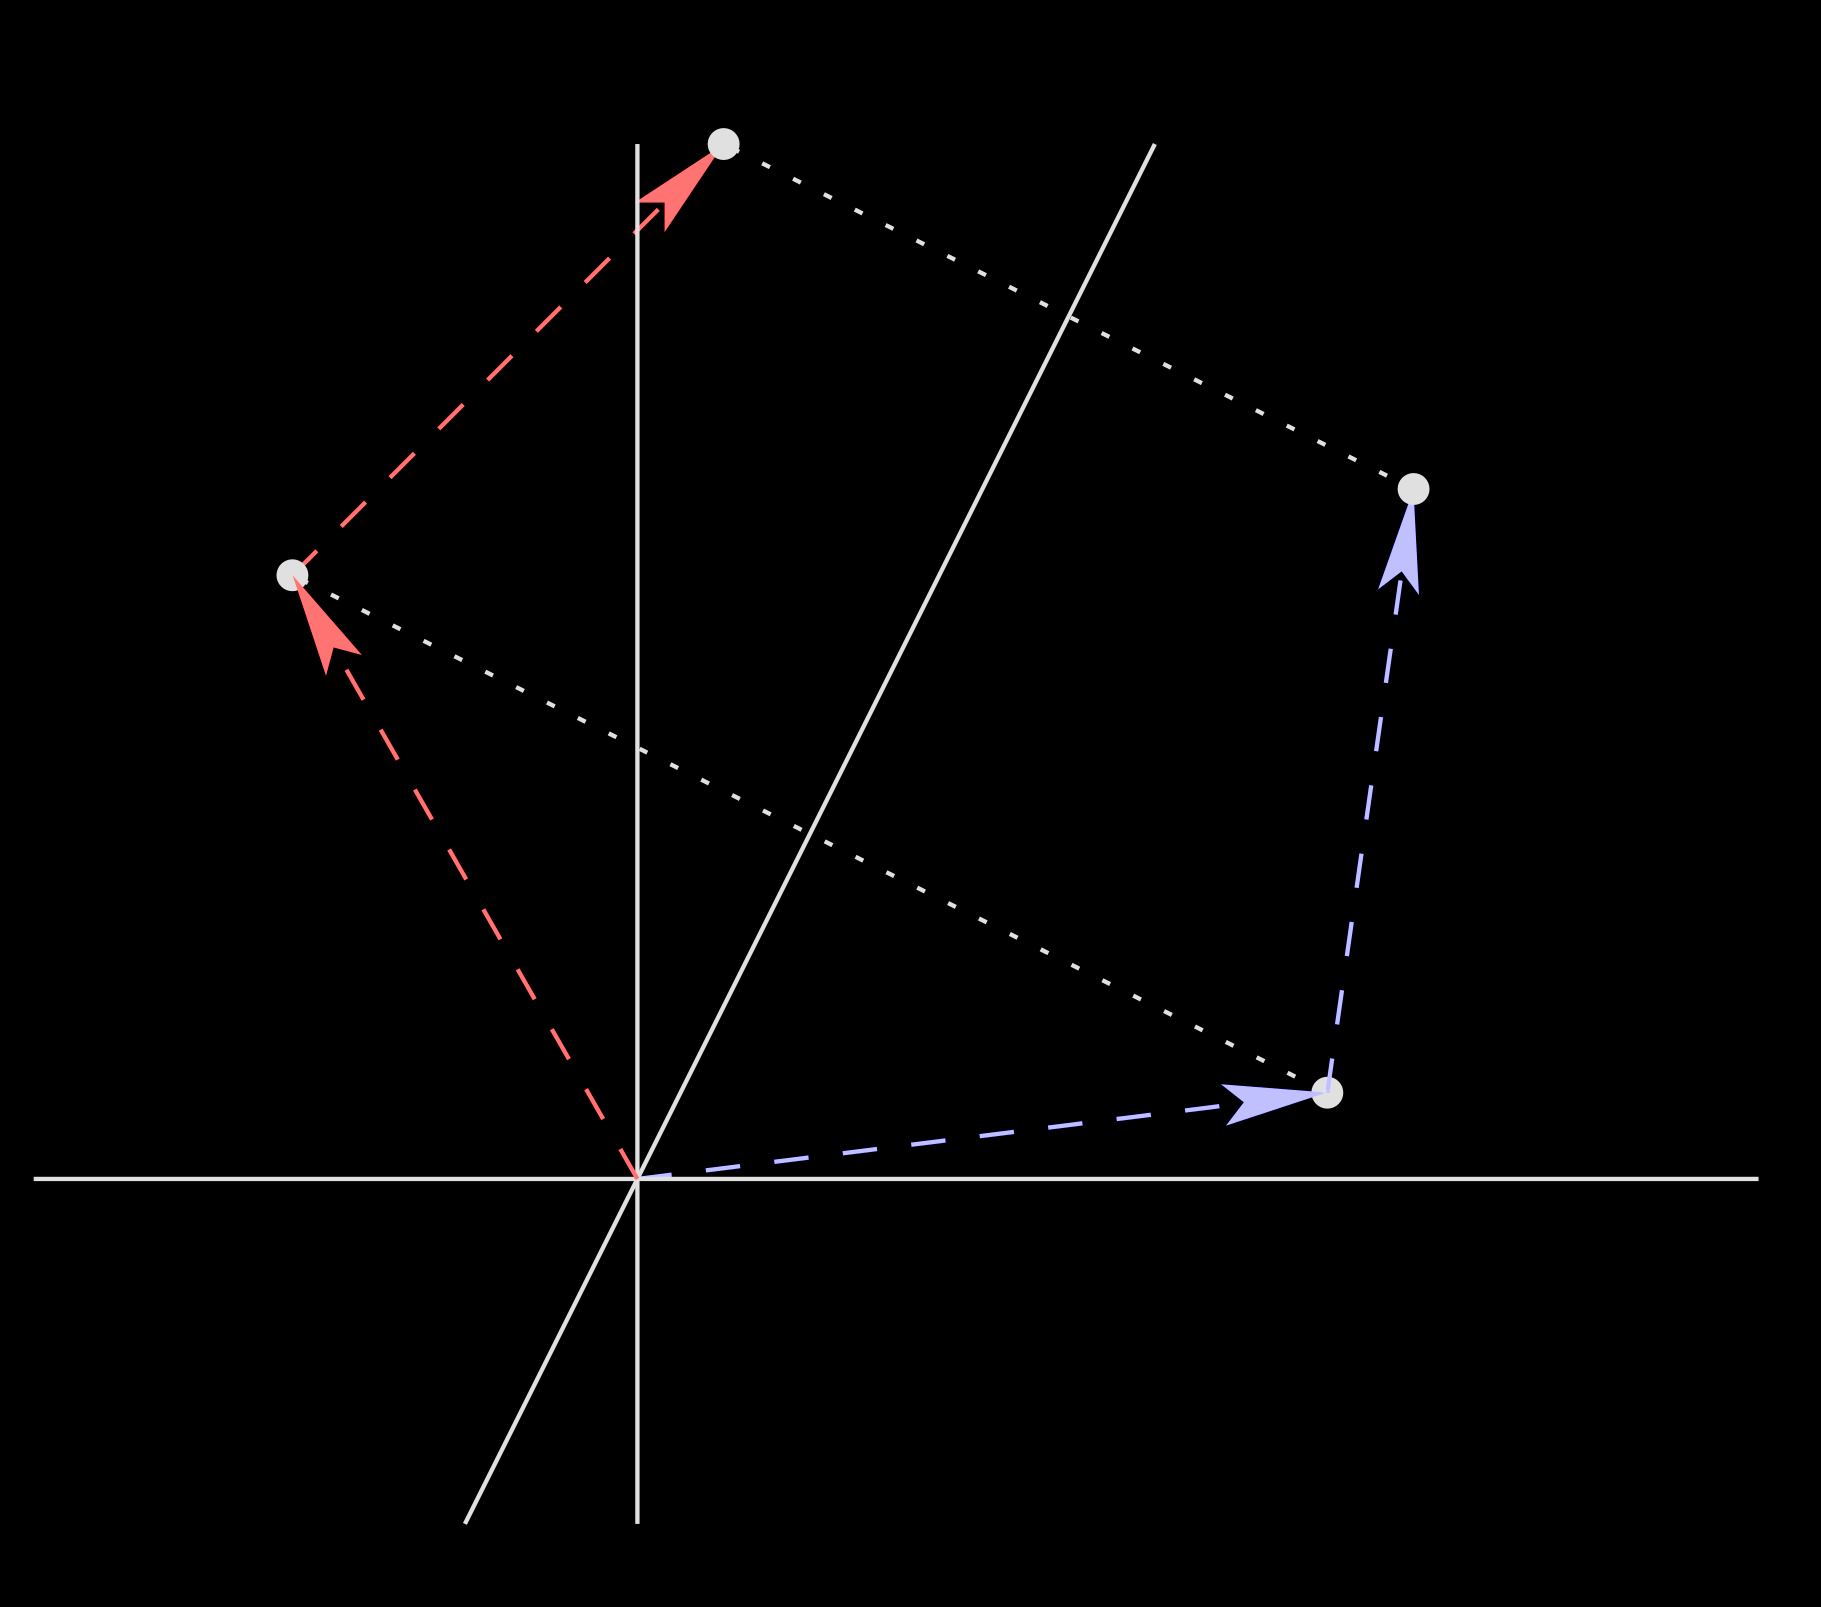
\includegraphics[scale=0.07]{figures/vectors-26b_copy.png}}
	    \put(3.65,1.25){\scriptsize{$y=mx$}}
	    \put(3.0,1.35){\scriptsize{$y$}}
	    \put(4.15,0.25){\scriptsize{$x$}}
	    \put(3.4,0.45){\scriptsize{\textcolor{blue}{$\vec{u}$}} }
	    \put(3.9,0.7){\scriptsize{\textcolor{blue}{$\vec{v}$}} }
	    \put(2.6,0.6){\scriptsize{\textcolor{red}{$Q_m(\vec{u})$}} }
	}
	\uncover<5->{
	    \put(2.6,1.2){\scriptsize{\textcolor{red}{$Q_m(\vec{v})$}} }
	    \put(3.65,1.25){\scriptsize{$y=mx$}}
	    \put(3.0,1.35){\scriptsize{$y$}}
	    \put(4.15,0.25){\scriptsize{$x$}}
	    \put(3.4,0.45){\scriptsize{\textcolor{blue}{$\vec{u}$}} }
	    \put(3.9,0.7){\scriptsize{\textcolor{blue}{$\vec{v}$}} }
	    \put(2.6,0.6){\scriptsize{\textcolor{red}{$Q_m(\vec{u})$}} }
	}
	\uncover<6->{
	    \put(2.5,0){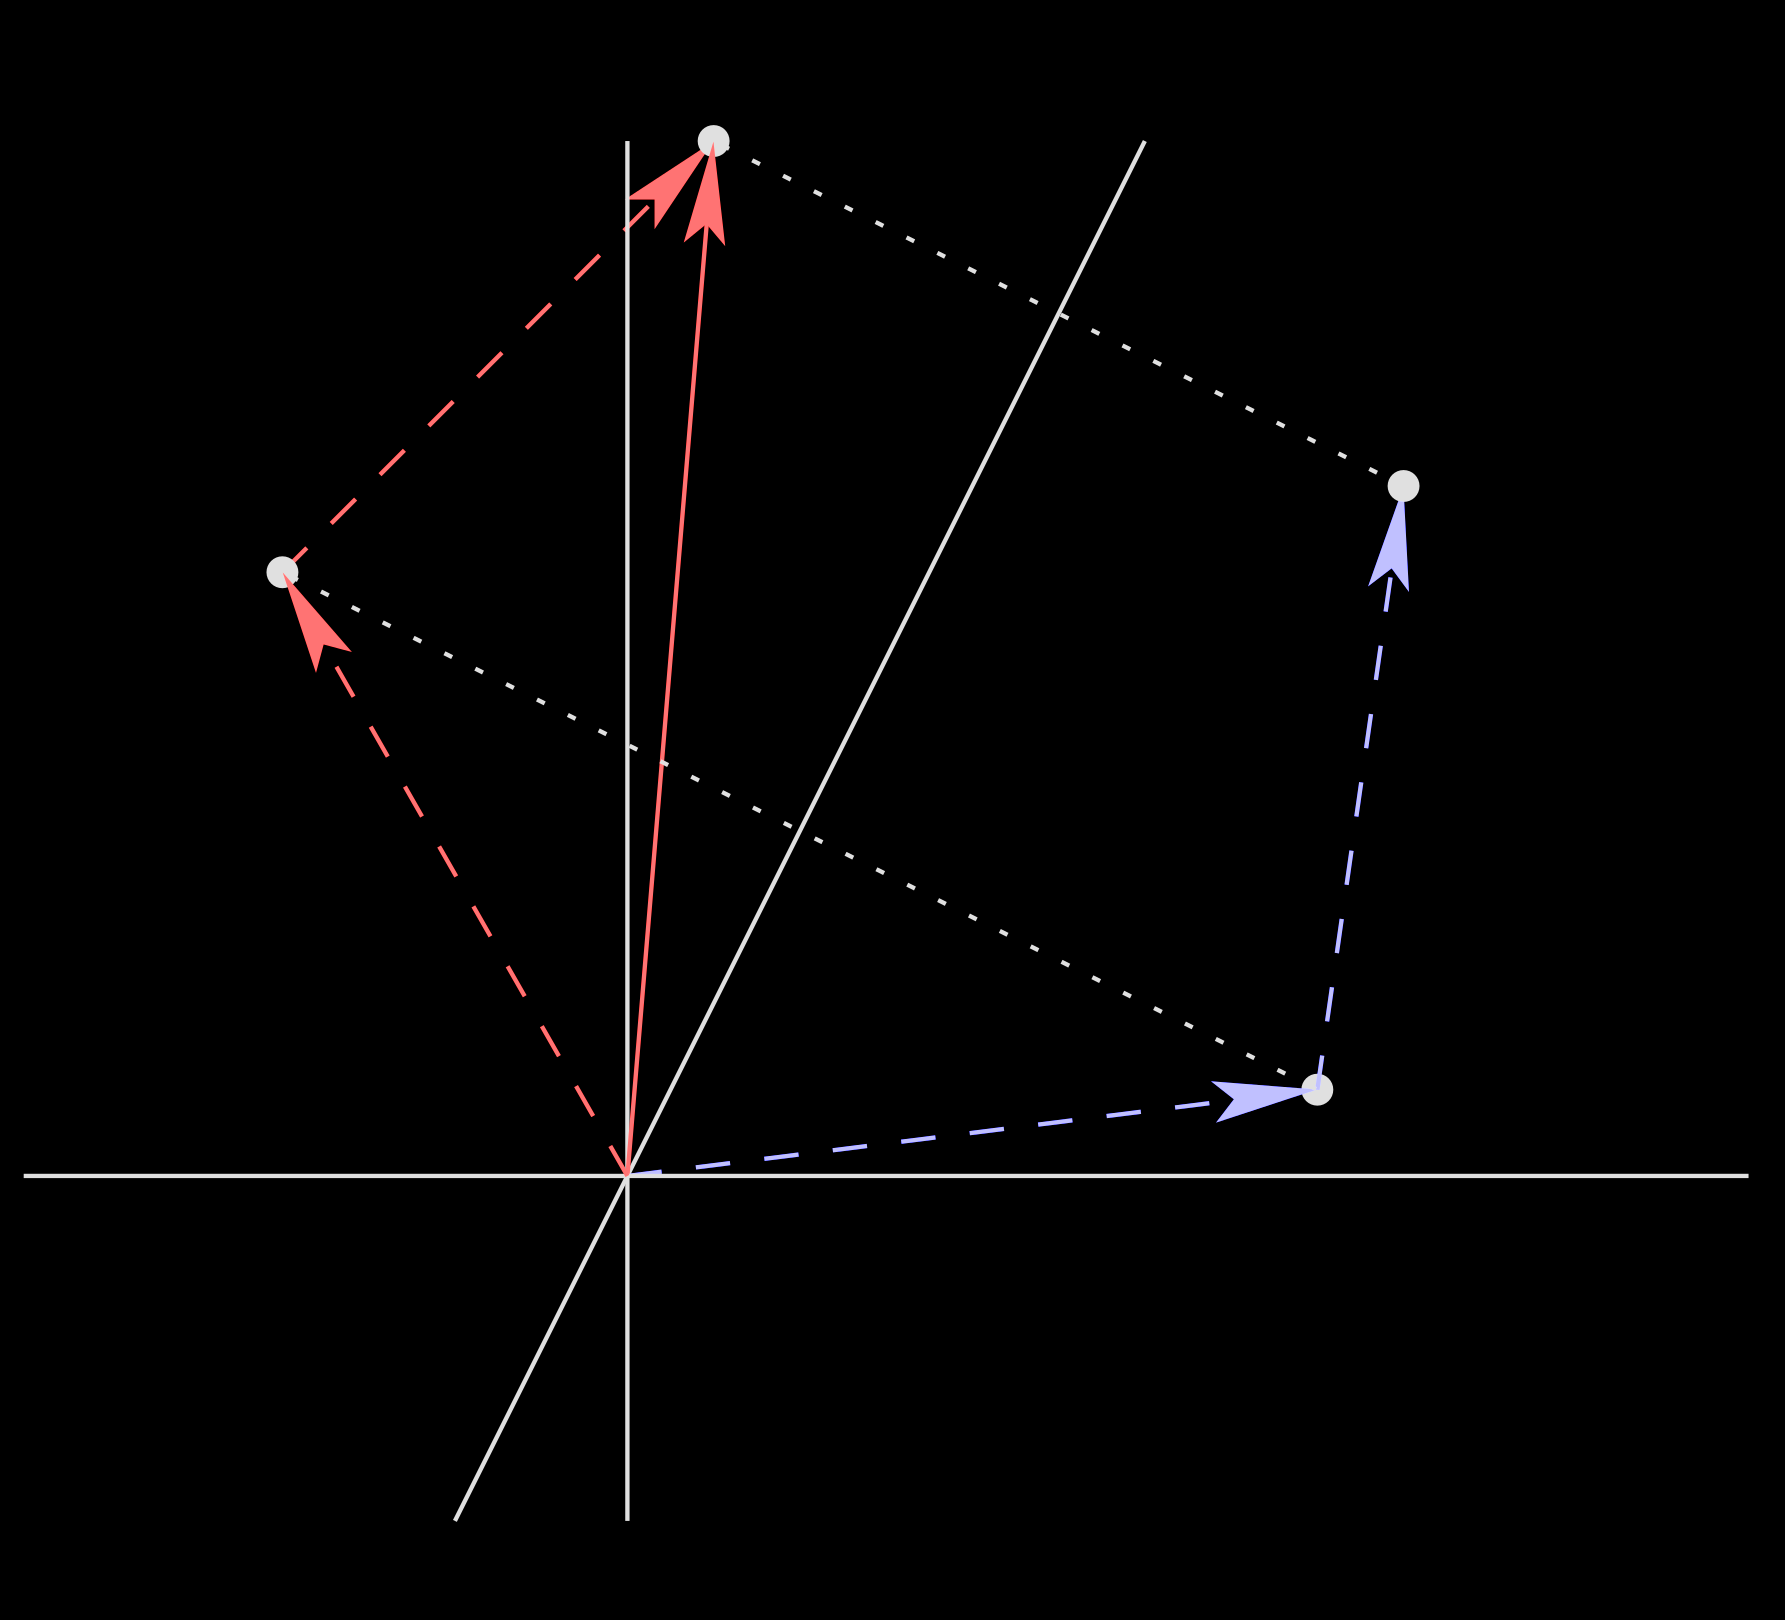
\includegraphics[scale=0.07]{figures/vectors-26c_copy.png}}
	    \put(3.65,1.25){\scriptsize{$y=mx$}}
	    \put(3.0,1.35){\scriptsize{$y$}}
	    \put(4.15,0.25){\scriptsize{$x$}}
	    \put(3.4,0.45){\scriptsize{\textcolor{blue}{$\vec{u}$}} }
	    \put(3.9,0.7){\scriptsize{\textcolor{blue}{$\vec{v}$}} }
	    \put(2.6,0.6){\scriptsize{\textcolor{red}{$Q_m(\vec{u})$}} }
	    \put(2.6,1.2){\scriptsize{\textcolor{red}{$Q_m(\vec{v})$}} }
	    \put(3.2,0.95){\scriptsize{\textcolor{red}{$Q_m(\vec{u}+\vec{v})$}} }
	}
	%\uncover<7->{
	%\put(2.5,0){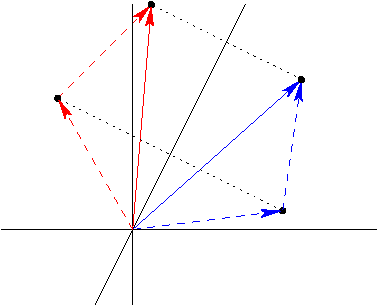
\includegraphics[scale=0.7]{figures/vectors-26.pdf}} }
    \end{picture}
    \bigskip

    \uncover<7->
    {The figure indicates that
	\alert{
    \[ Q_m(\vec{u}) + Q_m(\vec{v})=Q_m(\vec{u}+\vec{v}),\] } }
    \uncover<8->
    {i.e., $Q_m$ preserves vector addition.}
    \end{example}
}
%-------------- end slide -------------------------------%}}}

%-------------- start slide -------------------------------%{{{ 40
\frame{
\begin{emptytitle}
Since $Q_m$ preserves addition and scalar multiplication,
\alert{$Q_m$ is a linear transformation, and hence a matrix transformation.}
\bigskip
\pause

The matrix that induces $Q_m$ can be found by computing
$Q_m(\vec{e}_1)$ and $Q_m(\vec{e}_2)$, where
\[
\vec{e}_1=\left[\begin{array}{c} 1 \\ 0 \end{array}\right]
~\quad\text{and}\quad
\vec{e}_2=\left[\begin{array}{c} 0 \\ 1 \end{array}\right].
\]
\end{emptytitle}
}
%-------------- end slide -------------------------------%}}}

%-------------- start slide -------------------------------%{{{ 41
\frame{
    \begin{block}{$Q_m(\vec{e}_1)$}
    % \textcolor{titletextcolour}{Example ($Q_m(\vec{e}_1)$)}\\[0.5em]

    \begin{picture}(4,1.5)
	\uncover<1>{
	    \put(1.3,0){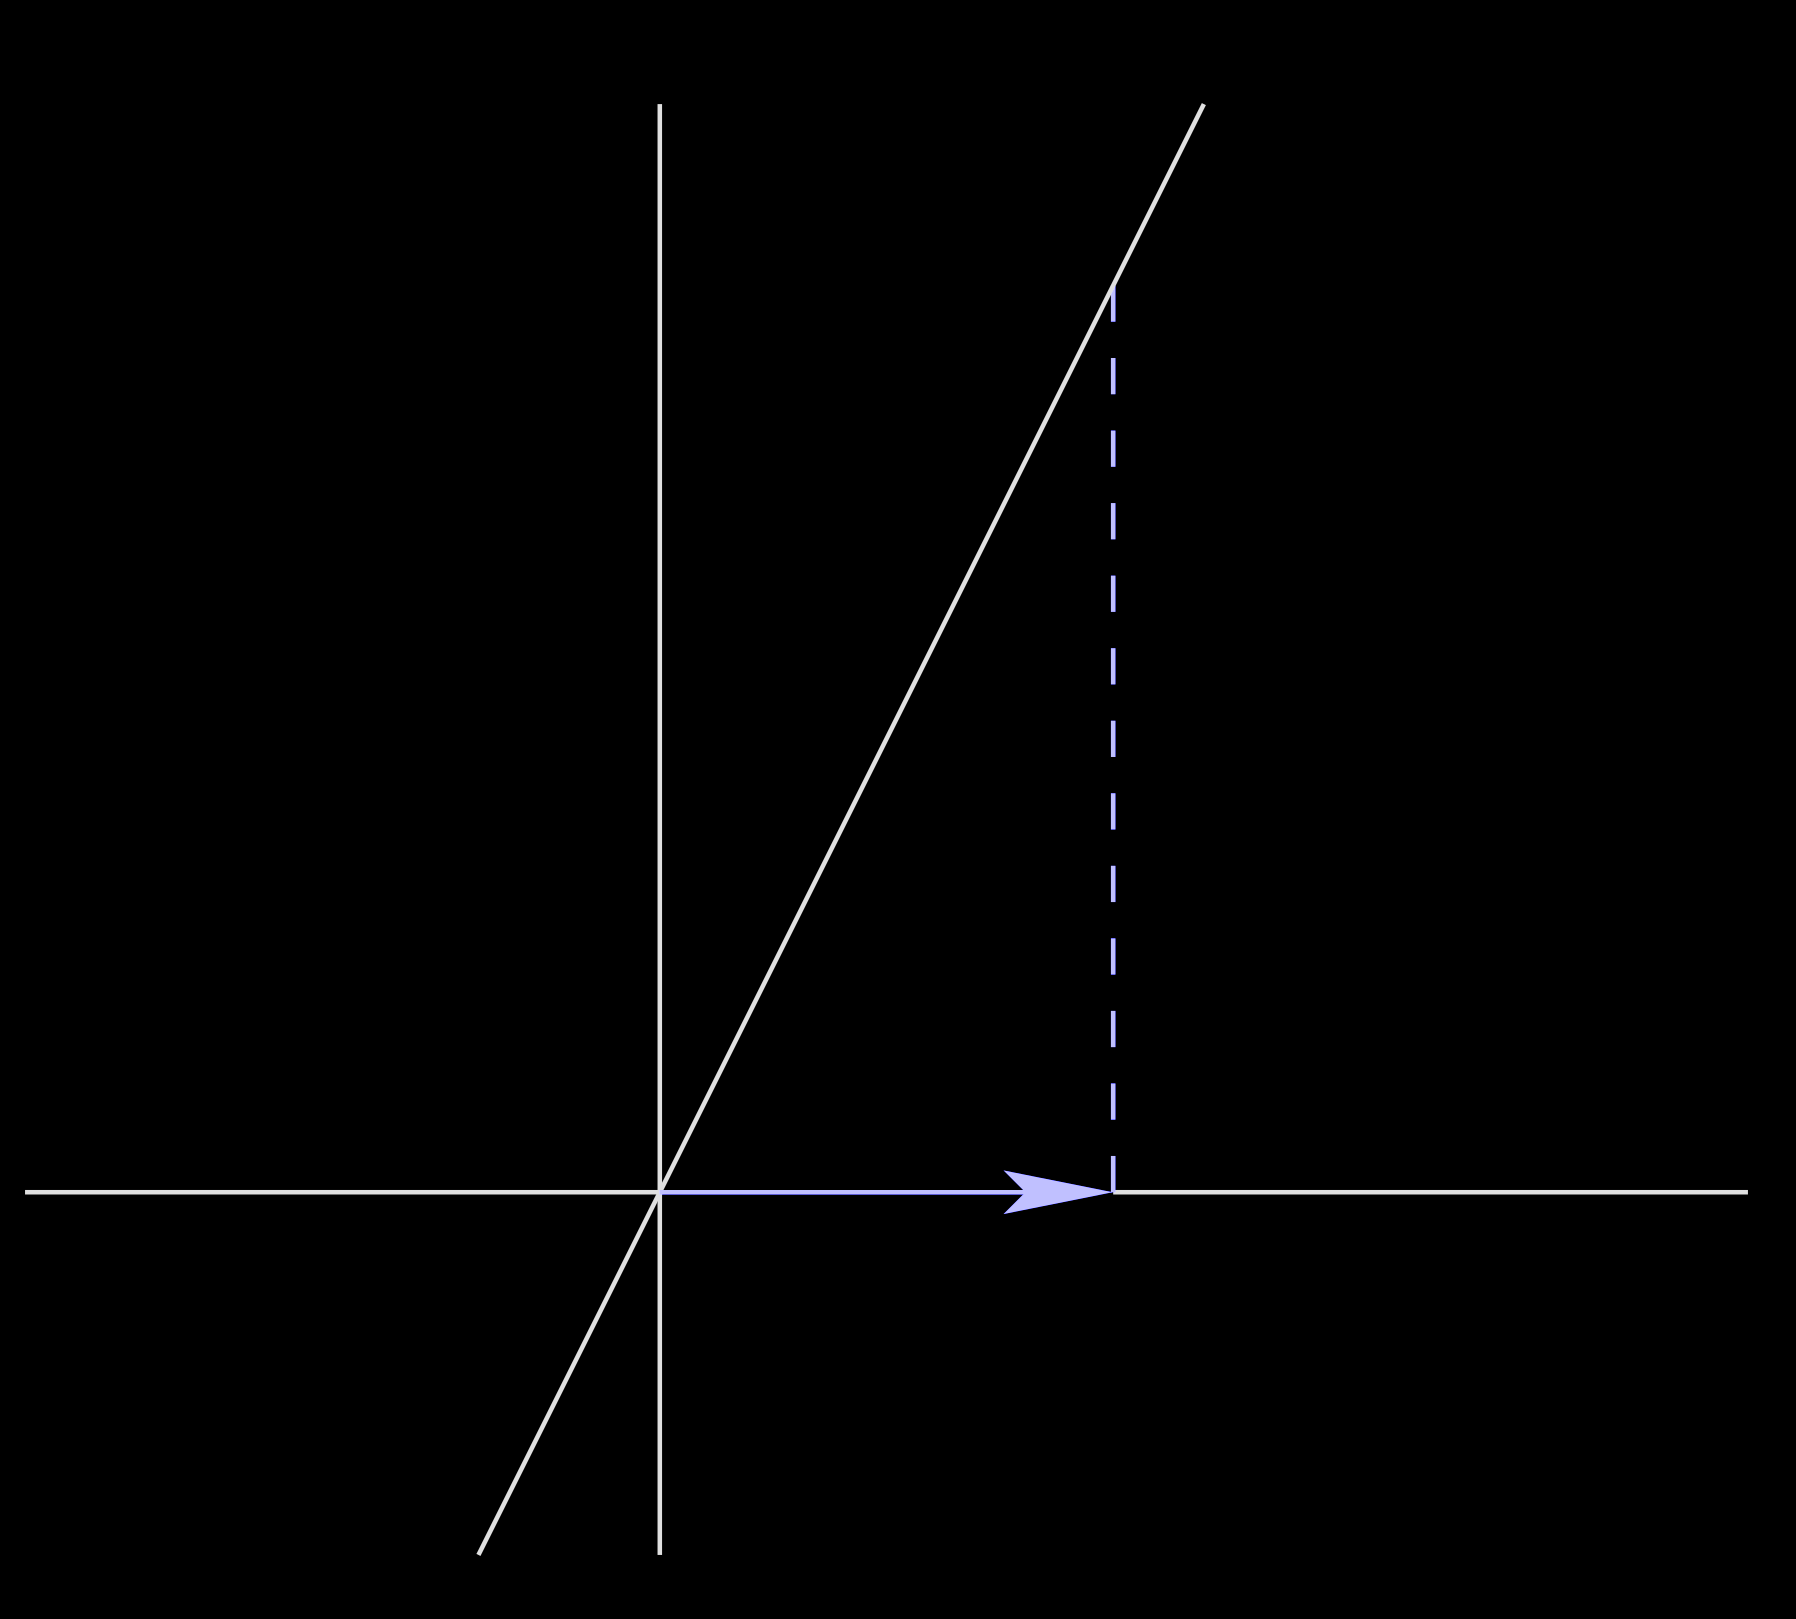
\includegraphics[scale=0.07]{figures/vectors-27a_copy.png}}
	\put(2.0,0.38){\tiny{$\theta$}} }
	\uncover<1->{
	    \put(2.45,1.25){\scriptsize{$y=mx$}}
	    \put(1.8,1.25){\scriptsize{$y$}}
	    \put(2.95,0.25){\scriptsize{$x$}}
	    \put(2.45,0.8){\scriptsize{\textcolor{blue}{$m$}} }
	    \put(2.1,0.25){\scriptsize{\textcolor{blue}{$1$}} }
	}
	\uncover<2>{
	    \put(1.3,0){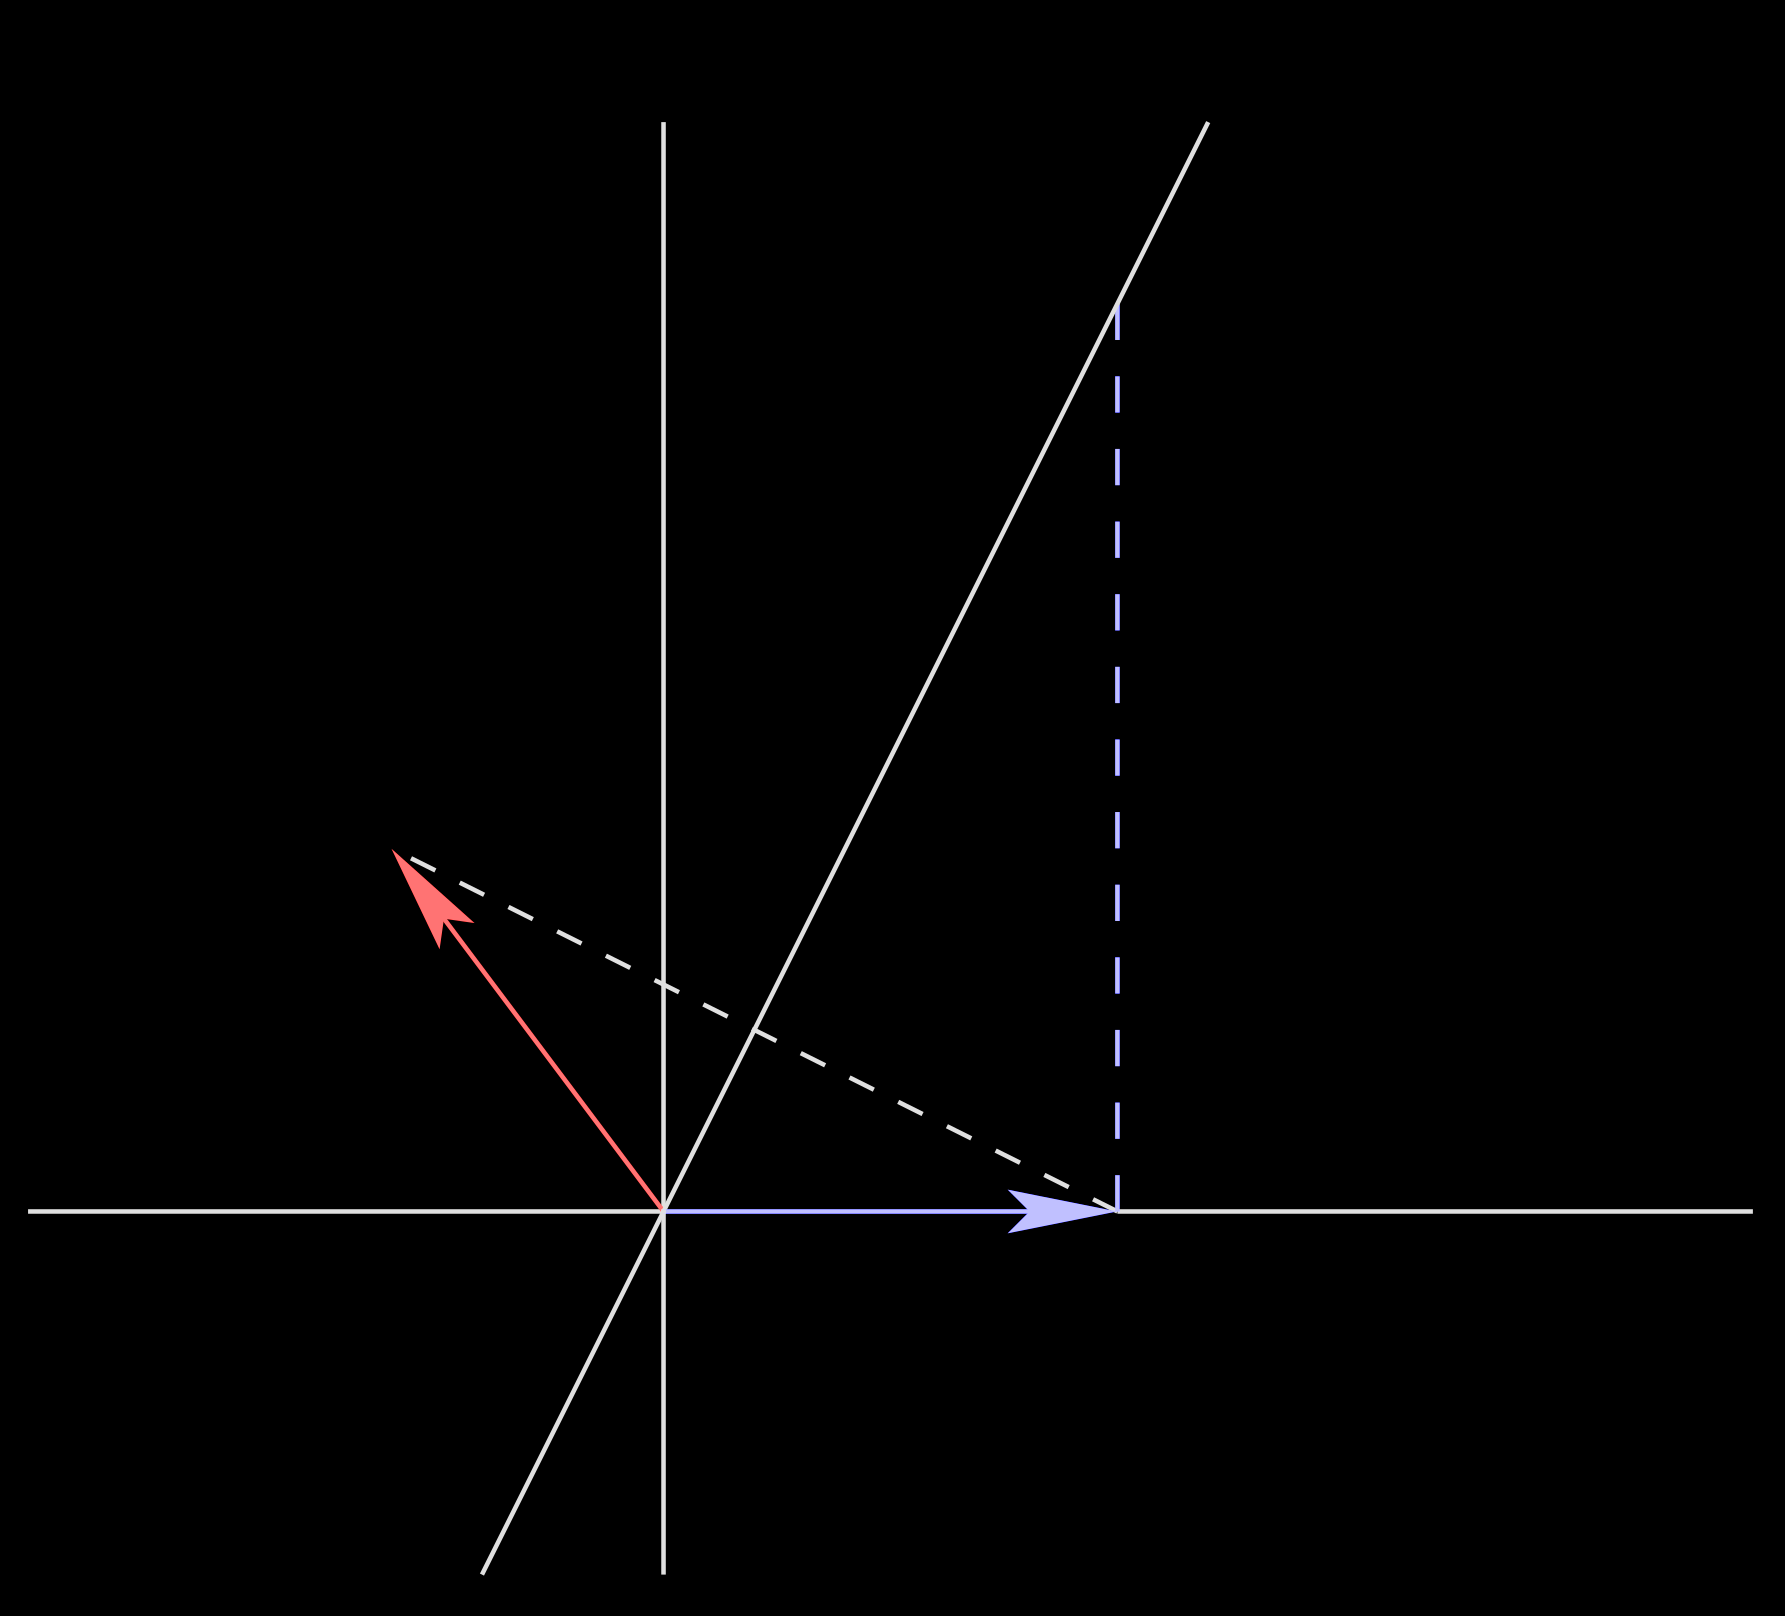
\includegraphics[scale=0.07]{figures/vectors-27b_copy.png}}
	    \put(2.45,1.25){\scriptsize{$y=mx$}}
	    \put(1.8,1.25){\scriptsize{$y$}}
	    \put(2.95,0.25){\scriptsize{$x$}}
	    \put(2.45,0.8){\scriptsize{\textcolor{blue}{$m$}} }
	    \put(2.1,0.25){\scriptsize{\textcolor{blue}{$1$}} }
	}
	\uncover<3->{
	    \put(1.3,0){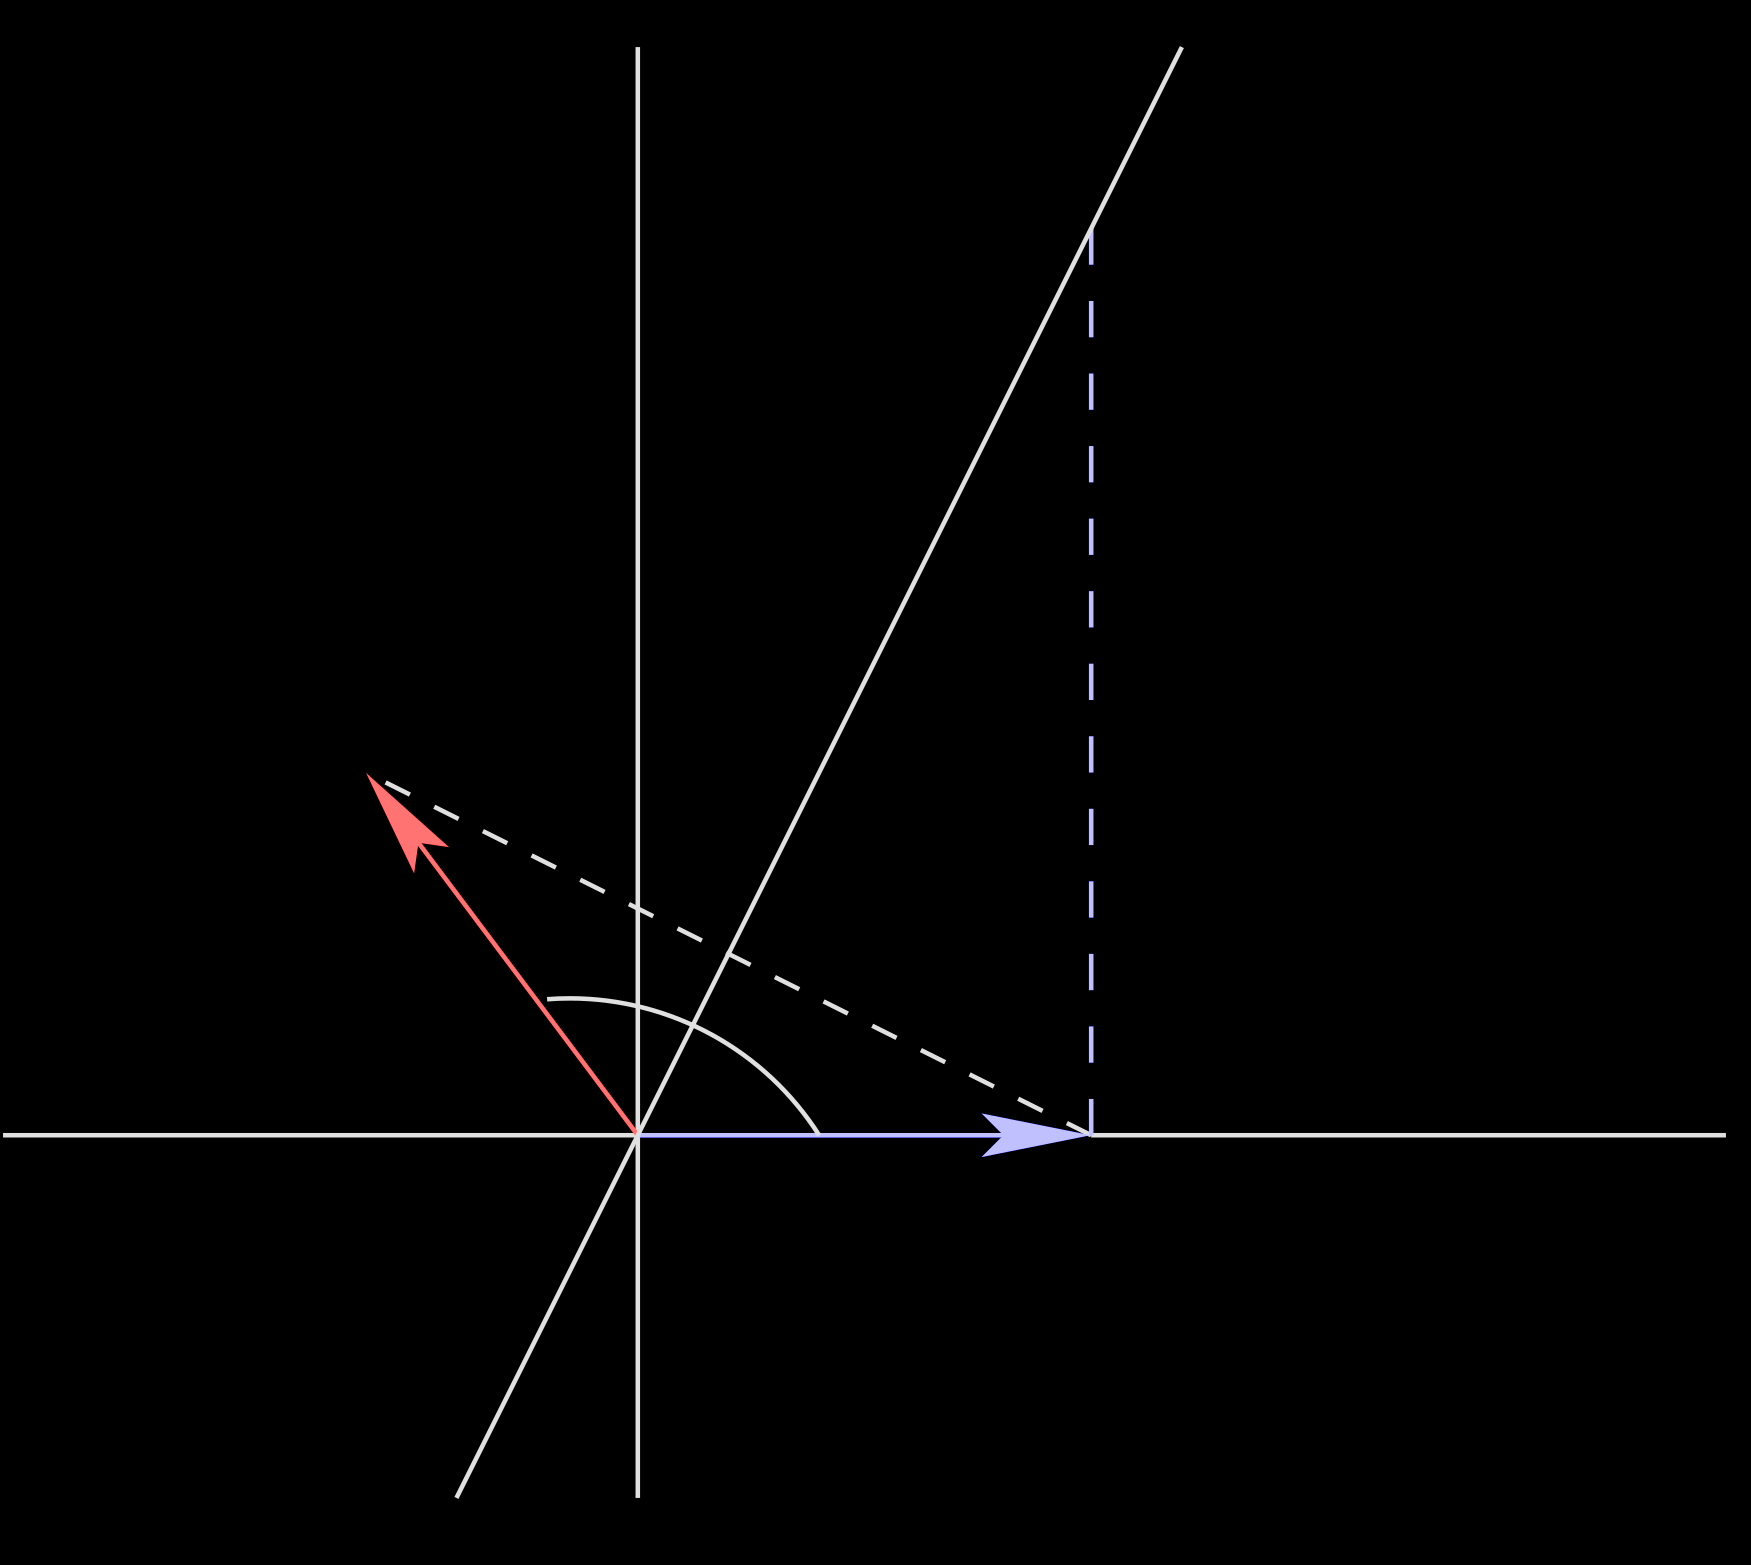
\includegraphics[scale=0.07]{figures/vectors-27c_copy.png}}
	    \put(2.45,1.25){\scriptsize{$y=mx$}}
	    \put(1.8,1.25){\scriptsize{$y$}}
	    \put(2.95,0.25){\scriptsize{$x$}}
	    \put(2.45,0.8){\scriptsize{\textcolor{blue}{$m$}} }
	    \put(2.1,0.25){\scriptsize{\textcolor{blue}{$1$}} }
	    \put(2.1,0.38){\tiny{$2\theta$}}
	}
    \end{picture}

    \[ \cos\theta = \frac{1}{\sqrt{1+m^2}}
	~\quad\text{and}\quad~
    \sin\theta = \frac{m}{\sqrt{1+m^2}} \]
    \[ \uncover<4->{
	    Q_m(\vec{e}_1) =\left[\begin{array}{c}
	\cos(2\theta) \\ \sin(2\theta) \end{array}\right]}
	\uncover<5->{
	    =\left[\begin{array}{c}
	\cos^2\theta-\sin^2\theta \\ 2\sin\theta \cos\theta \end{array}\right]}
	\uncover<6->{
	    =\frac{1}{1+m^2}\left[\begin{array}{c}
	1-m^2 \\ 2m \end{array}\right]}
    \]
    \end{block}
}
%-------------- end slide -------------------------------%}}}

%-------------- start slide -------------------------------%{{{ 42
\frame{
    \begin{block}{ $Q_m(\vec{e}_2)$ }
    % \textcolor{titletextcolour}{Example ($Q_m(\vec{e}_2)$)}\\[0.5em]
    \begin{picture}(4,1.5)
	\uncover<1>{
	\put(1.3,0){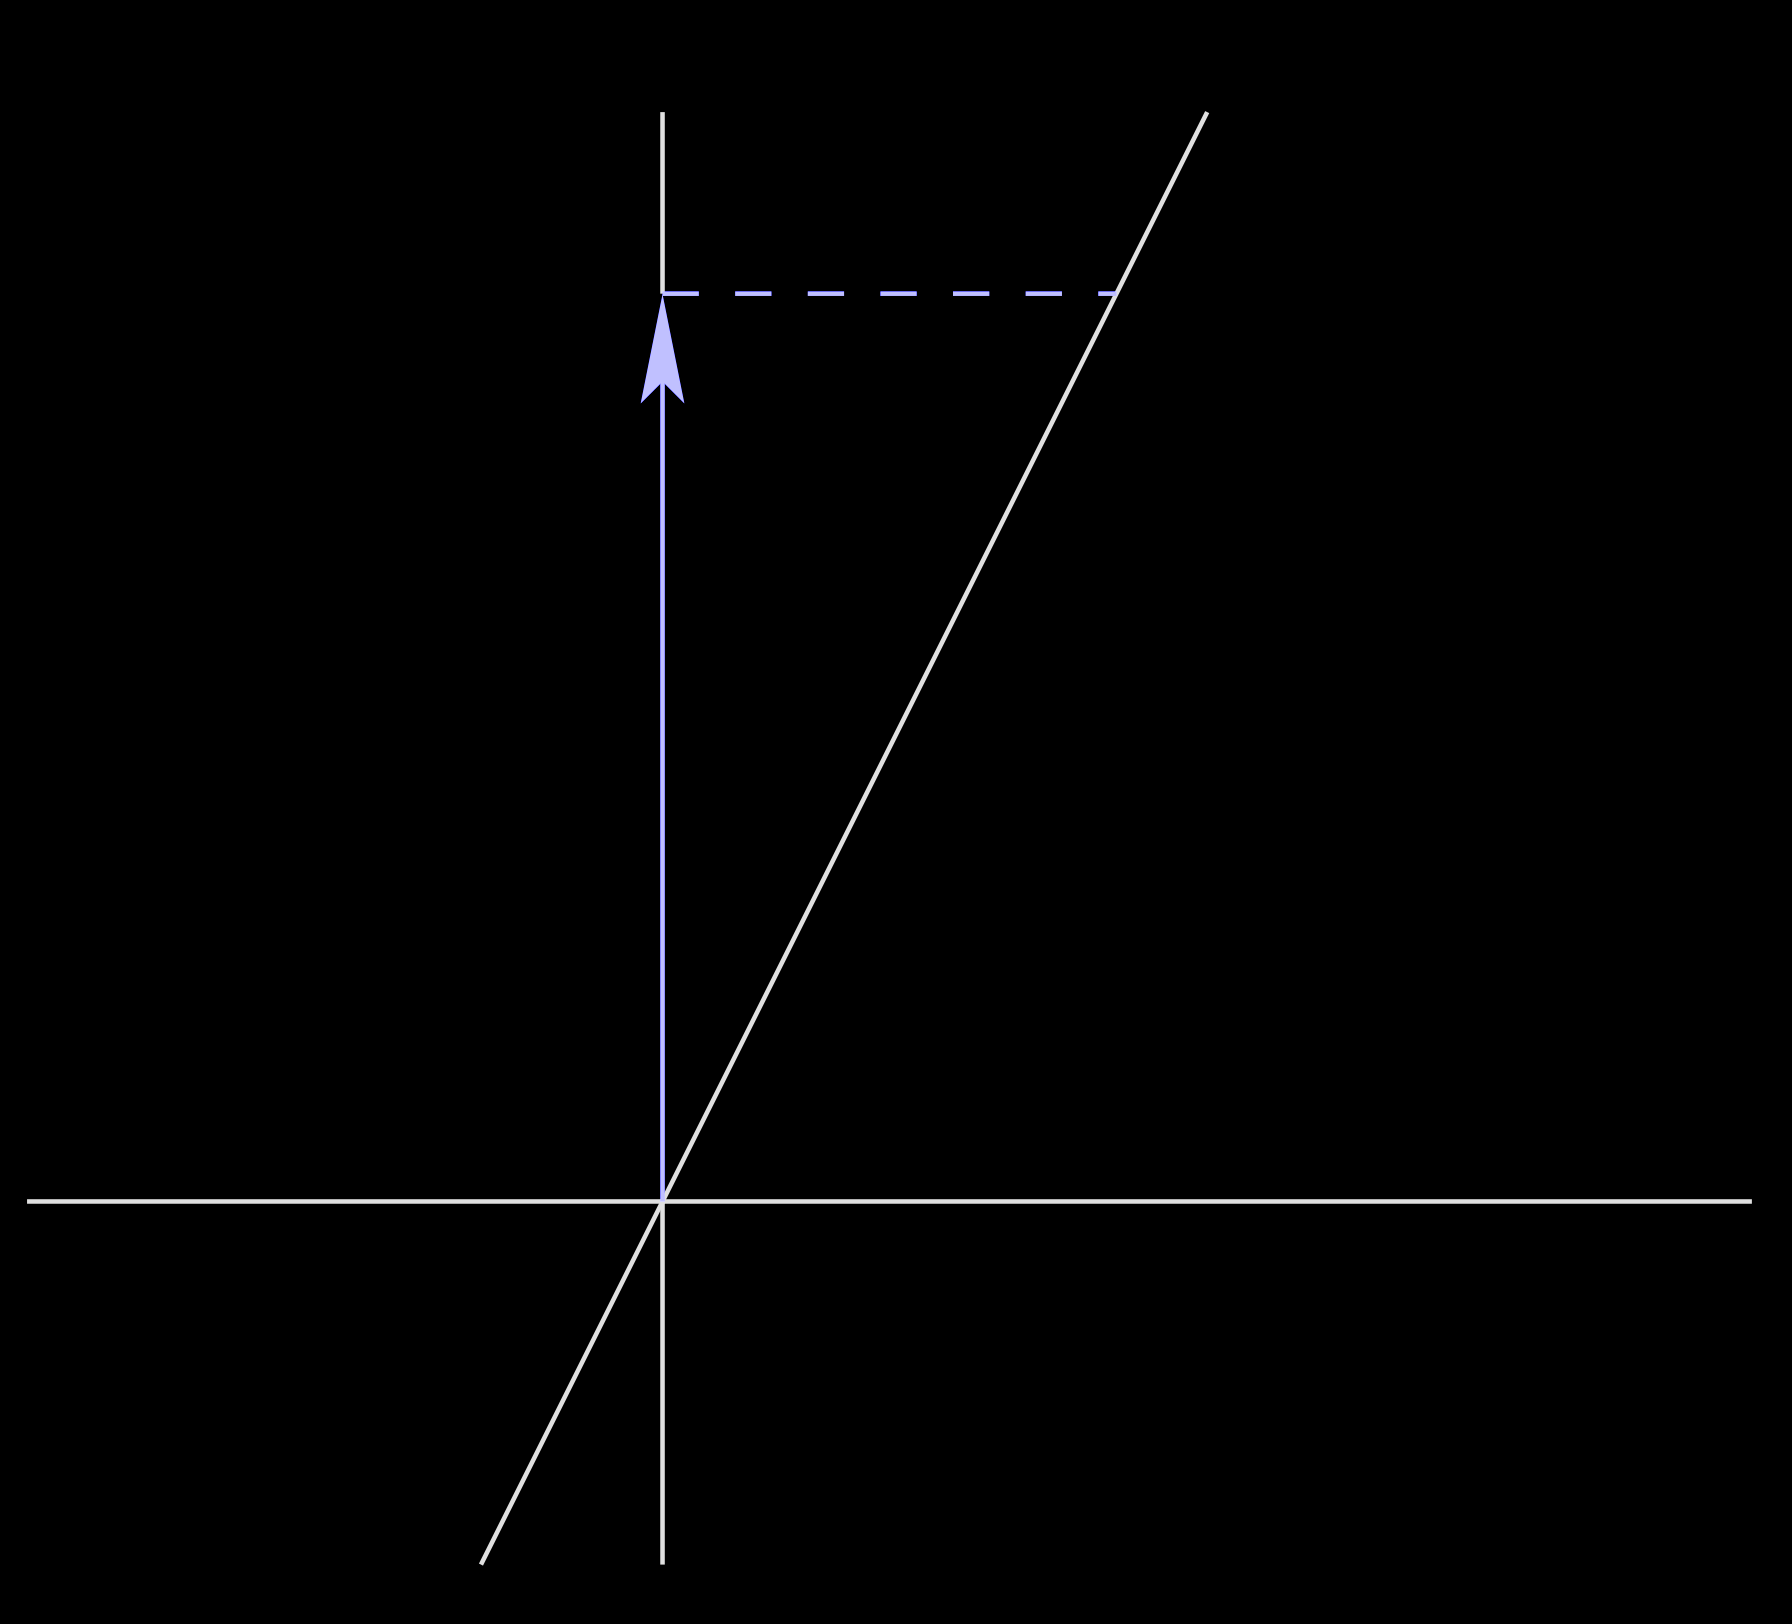
\includegraphics[scale=0.065]{figures/vectors-28a_copy.png}} }
	\uncover<1->{
	    \put(2.45,1.25){\scriptsize{$y=mx$}}
	    \put(1.8,1.25){\scriptsize{$y$}}
	    \put(2.95,0.25){\scriptsize{$x$}}
	    \put(1.91,0.5){\tiny{$\theta$}}
	    \put(1.75,0.8){\scriptsize{\textcolor{blue}{$1$}} }
	    \put(2.1,1.35){\scriptsize{\textcolor{blue}{$\frac{1}{m}$}} }
	}
	\uncover<2>{
	    \put(1.3,0){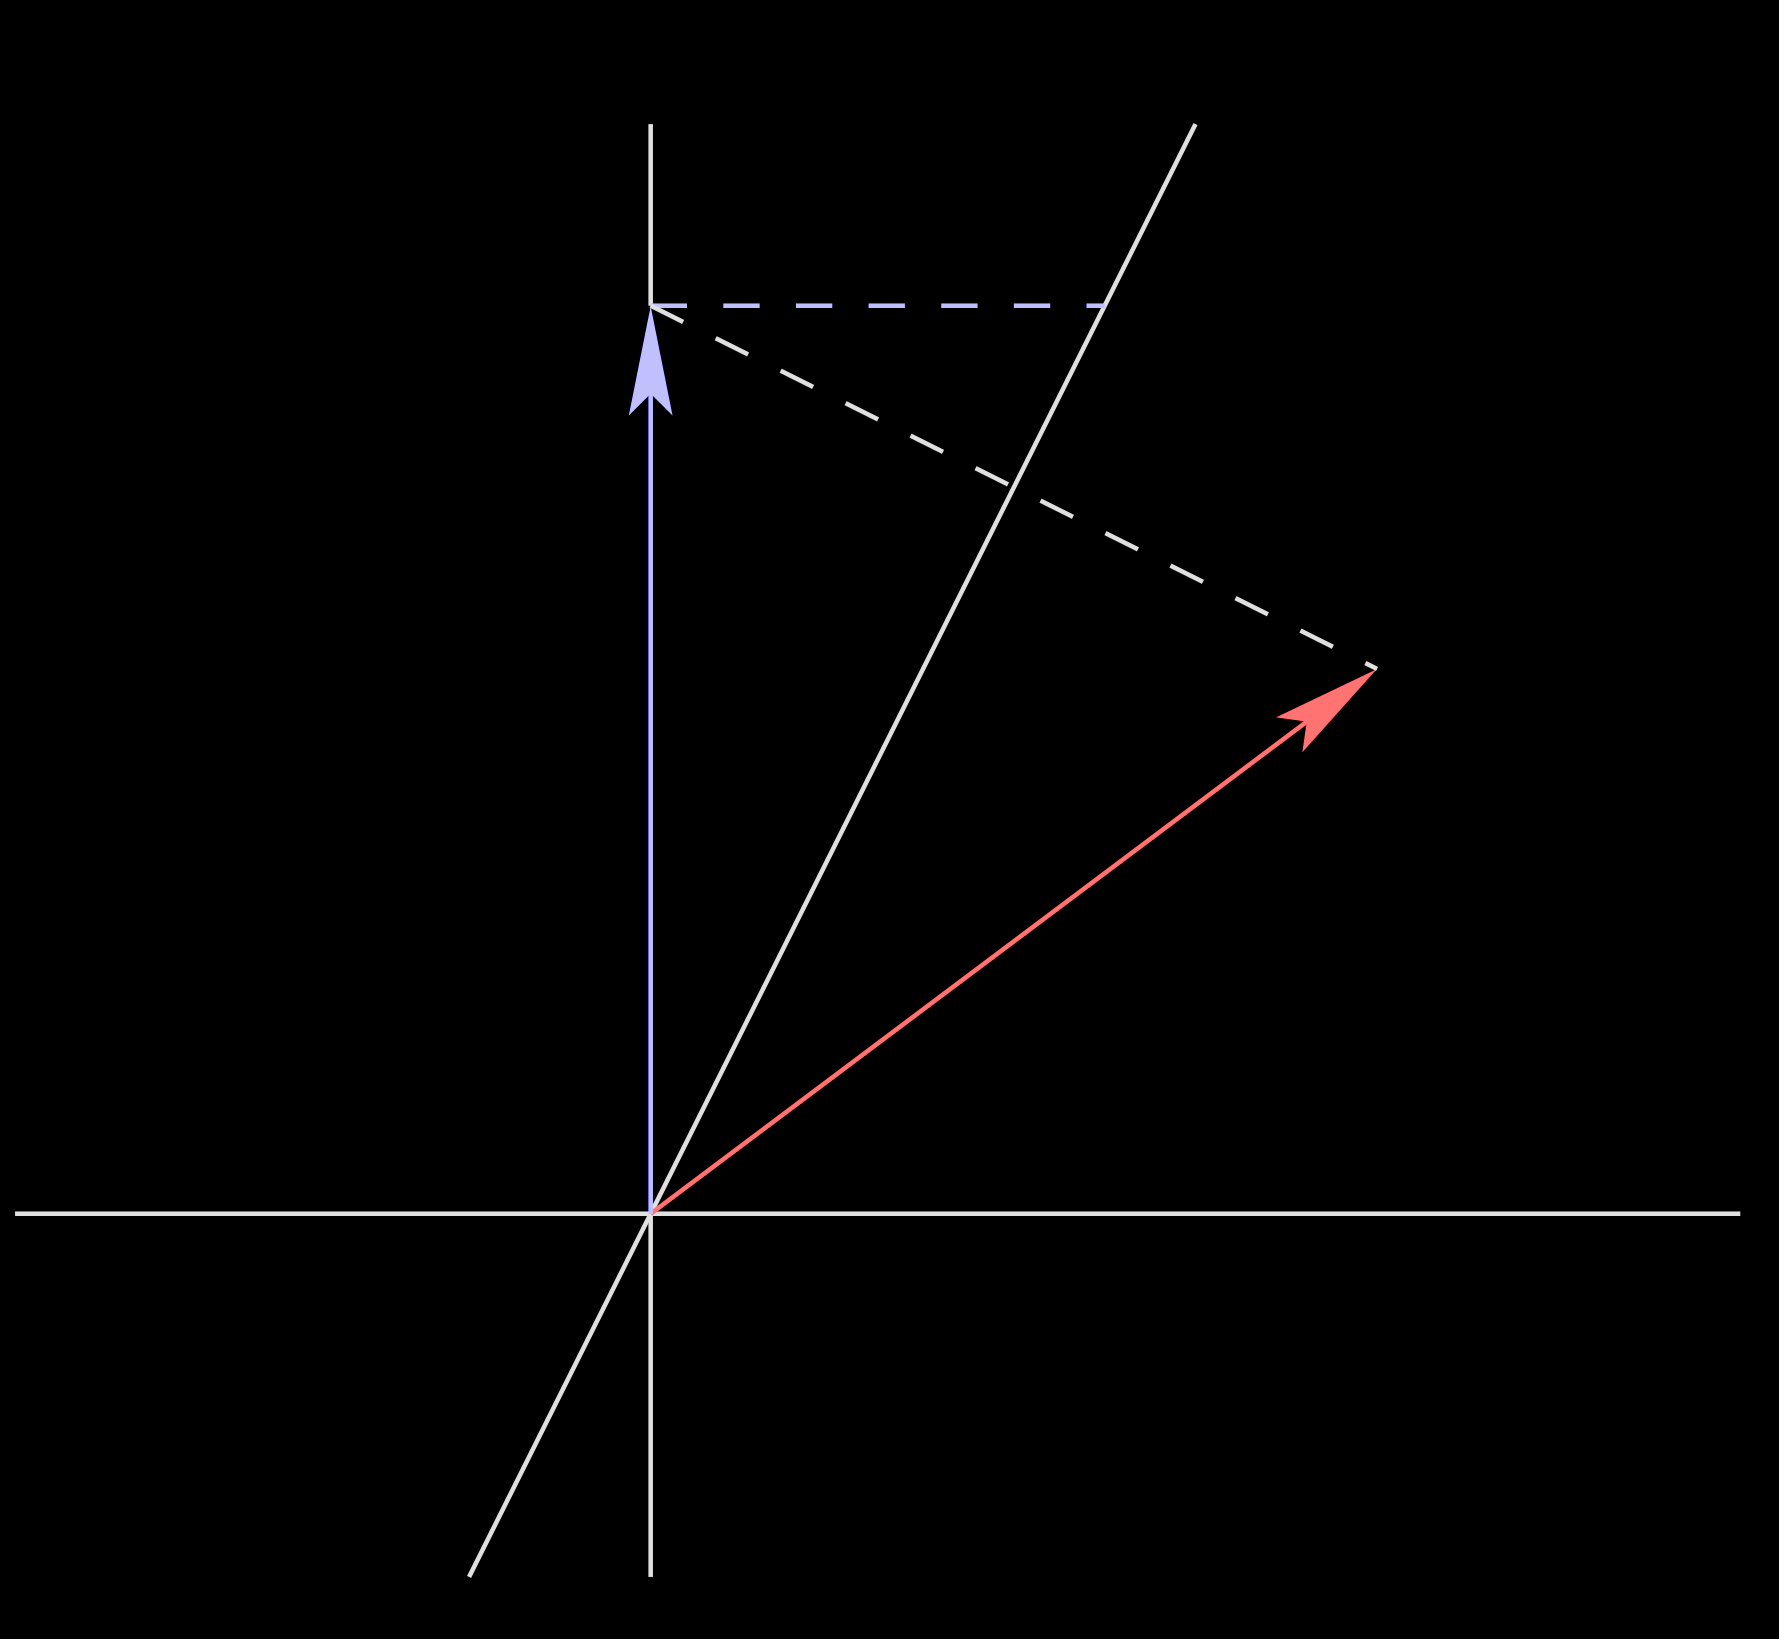
\includegraphics[scale=0.065]{figures/vectors-28b_copy.png}}
	    \put(2.45,1.25){\scriptsize{$y=mx$}}
	    \put(1.8,1.25){\scriptsize{$y$}}
	    \put(2.95,0.25){\scriptsize{$x$}}
	    \put(1.91,0.5){\tiny{$\theta$}}
	    \put(1.75,0.8){\scriptsize{\textcolor{blue}{$1$}} }
	    \put(2.1,1.35){\scriptsize{\textcolor{blue}{$\frac{1}{m}$}} }
	}
	\uncover<3->{
	    \put(1.3,0){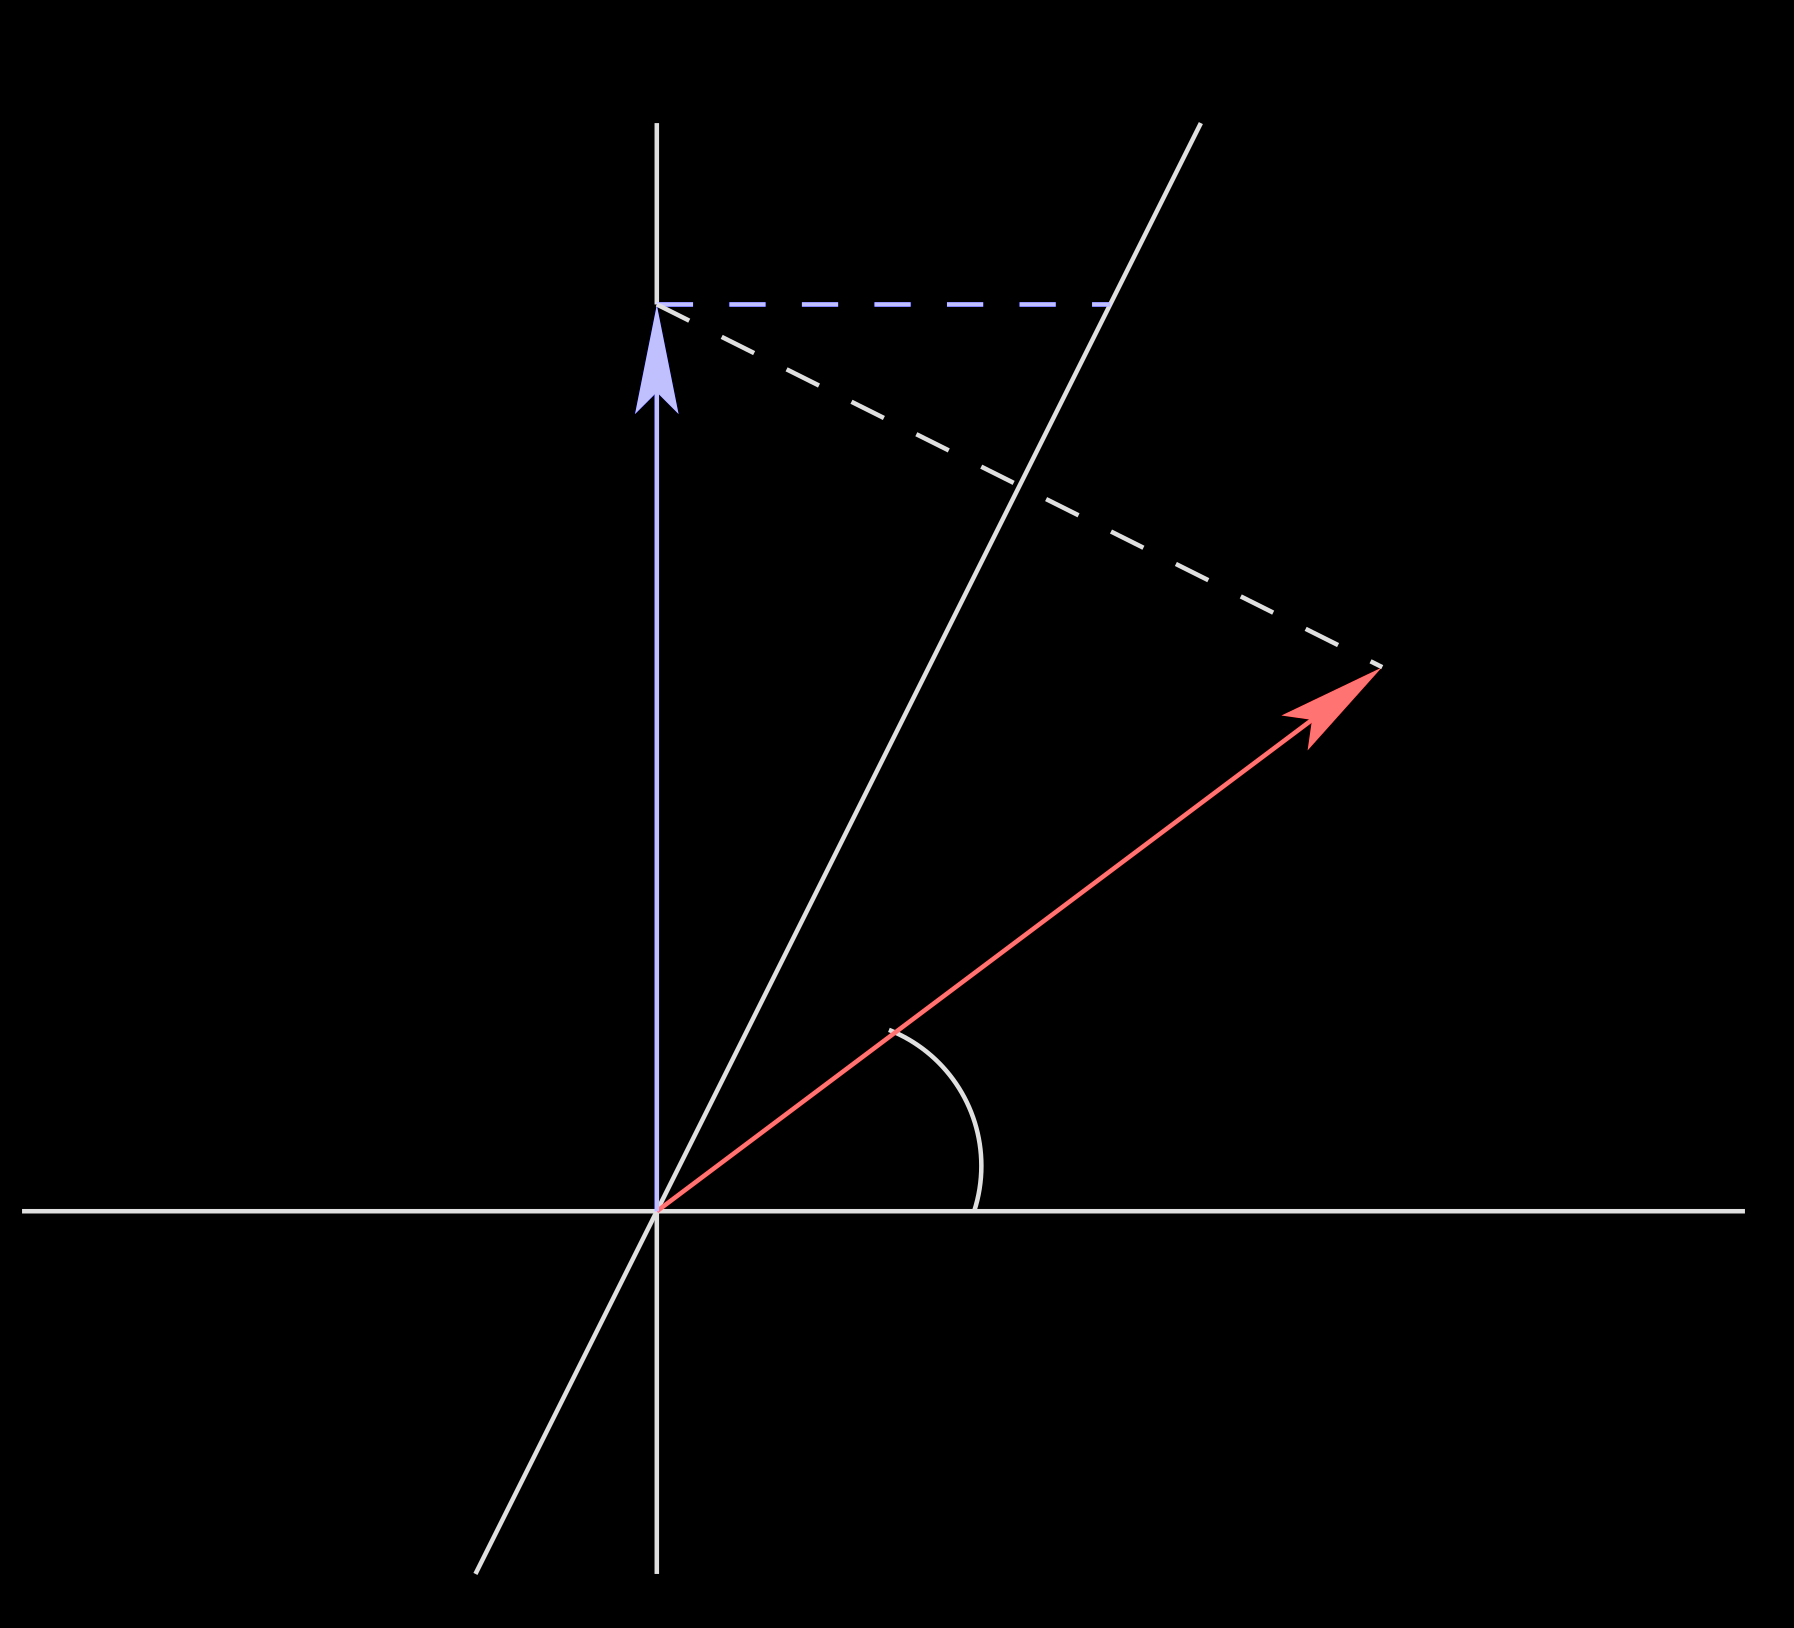
\includegraphics[scale=0.065]{figures/vectors-28c_copy.png}}
	    \put(2.26,0.45){\tiny{$\frac{\pi}{2}-2\theta$}}
	    \put(2.45,1.25){\scriptsize{$y=mx$}}
	    \put(1.8,1.25){\scriptsize{$y$}}
	    \put(2.95,0.25){\scriptsize{$x$}}
	    \put(1.91,0.5){\tiny{$\theta$}}
	    \put(1.75,0.8){\scriptsize{\textcolor{blue}{$1$}} }
	    \put(2.1,1.35){\scriptsize{\textcolor{blue}{$\frac{1}{m}$}} }
    }
    \end{picture}

    \uncover<1->{
	\[ \cos\theta = \frac{m}{\sqrt{1+m^2}}
	    ~\quad\text{and}\quad~
    \sin\theta = \frac{1}{\sqrt{1+m^2}} \]}
    \begin{eqnarray*}
	\uncover<4->{
	    Q_m(\vec{e}_2) & = & \left[\begin{array}{c}
	\cos(\frac{\pi}{2}-2\theta) \\ \sin(\frac{\pi}{2}-2\theta) \end{array}\right]}
	\uncover<5->{
	    =\left[\begin{array}{c}
		    \cos\frac{\pi}{2} \cos(2\theta)+\sin\frac{\pi}{2} \sin(2\theta) \\
		    \sin\frac{\pi}{2} \cos(2\theta)-\cos\frac{\pi}{2} \sin(2\theta) \\
	\end{array}\right]} \\
	\uncover<6->{
		     & = & \left[\begin{array}{c}
		 \sin(2\theta) \\ \cos(2\theta) \end{array}\right]}
		 \uncover<7->{
		     =\left[\begin{array}{c}
		 2\sin\theta \cos\theta \\ \cos^2\theta-\sin^2\theta  \end{array}\right]}
		 \uncover<8->{
		     =\frac{1}{1+m^2}\left[\begin{array}{c}
		 2m \\ m^2-1 \end{array}\right]}
		\end{eqnarray*}
    \end{block}
}
%-------------- end slide -------------------------------%}}}

%-------------- start slide -------------------------------%{{{ 43
\begin{frame}[fragile]
\begin{emptytitle}
    Alternatively, we can use the following relation to find $Q_m:$
    \begin{align*}
	Q_m = R_\theta \circ Q_0 \circ R_{-\theta}
    \end{align*}
    \pause
    \bigskip
    \begin{align*}
        R_\theta \sim
	\begin{bmatrix} \cos(\theta) & -\sin(\theta)\cr \sin(\theta) &
	\cos(\theta) \end{bmatrix},\qquad
	    Q_0 \sim \begin{bmatrix} 1 & 0 \cr 0 & -1 \end{bmatrix}
	    \quad
	R_{-\theta} \sim
	\begin{bmatrix} \cos(\theta) & \sin(\theta)\cr -\sin(\theta) &
	\cos(\theta) \end{bmatrix},\qquad
    \end{align*}
    \bigskip

    \pause
    Then multiply these three matrices ...
\end{emptytitle}
\end{frame}
%-------------- end slide -------------------------------%}}}

%-------------- start slide -------------------------------%{{{ 44
\frame{
\begin{block}{The Matrix for Reflection in $y=mx$}
The transformation $Q_m:\RR^2\rightarrow\RR^2$,
reflection in the line $y=mx$,
is a linear transformation and is induced by the matrix
\[ \frac{1}{1+m^2}
\left[\begin{array}{cc}
1-m^2 & 2m \\ 2m & m^2-1
\end{array}\right].\]
\end{block}
}
%-------------- end slide -------------------------------%}}}

%-------------- start slide -------------------------------%{{{ 45
\frame{
\begin{problem}[ Multiple Actions ]
    Find the rotation or reflection that equals reflection in the
    $x$-axis followed by rotation through an angle of $\frac{\pi}{2}$.
\end{problem}
\vfill
\pause
\begin{solution}
    Let $Q_0$ denote the reflection in the $x$-axis, and $R_{\frac{\pi}{2}}$ denote the rotation through an angle of $\frac{\pi}{2}$. We want to find the matrix for the transformation
    $R_{\frac{\pi}{2}}\circ Q_0$.

    \pause
    $Q_0$ is induced by
    $A= \left[\begin{array}{rr}
    1 & 0 \\ 0 & -1
    \end{array}\right]$, and
    $R_{\frac{\pi}{2}}$ is induced by
    \[
    B=\left[\begin{array}{rr}
    \cos\frac{\pi}{2} & -\sin\frac{\pi}{2} \\
    \sin\frac{\pi}{2} & \cos\frac{\pi}{2}
    \end{array}\right]
    =
    \left[\begin{array}{rr}
    0 & -1 \\ 1 & 0
    \end{array}\right]
    \]
\end{solution}
}
%-------------- end slide -------------------------------%}}}

%-------------- start slide -------------------------------%{{{ 46
\frame{
\begin{solution}
    Hence $R_{\frac{\pi}{2}}\circ Q_0$ is induced by
    \[ BA =
    \left[\begin{array}{rr} 0 & -1 \\ 1 & 0 \end{array}\right]
    \left[\begin{array}{rr} 1 & 0  \\ 0 & -1 \end{array}\right] =
    \left[\begin{array}{rr} 0 & 1  \\ 1 & 0 \end{array}\right].\]

    \pause

    Notice that
    $BA= \left[\begin{array}{rr} 0 & 1 \\ 1 & 0 \end{array}\right]$
    is a \alert{reflection} matrix.

    \pause
    \begin{center}
    \alert{\Large How do we know this?}
    \end{center}
\end{solution}
}
%-------------- end slide -------------------------------%}}}

%-------------- start slide -------------------------------%{{{ 47
\frame{
\begin{solution}[continued]
    Compare $BA$ to
    \[ Q_m = \frac{1}{1+m^2}
    \left[\begin{array}{cc}
    1-m^2 & 2m \\ 2m & m^2-1
    \end{array}\right]
    \]
    \pause
    Now, since $1-m^2=0$, we know that $m=1$ or $m=-1$.
    But $\frac{2m}{1+m^2}=1>0$, so $m>0$, implying $m=1$.
    \medskip
    \pause

    Therefore,
    \[ R_{\frac{\pi}{2}}\circ Q_0 = Q_1,\]
    reflection in the line $y=x$.
    \myQED
\end{solution}
}
%-------------- end slide -------------------------------%}}}

%-------------- start slide -------------------------------%{{{ 48
\frame{
\begin{problem}[Reflection followed by Reflection]
    Find the rotation or reflection that equals reflection in the
    line $y=-x$ followed by reflection in the $y$-axis.
\end{problem}
\vfill
\pause
\begin{solution}
    We must find the matrix for the transformation
    $Q_Y\circ Q_{-1}$.
    \bigskip
    \pause

    $Q_{-1}$ is induced by
    \[ A= \frac{1}{2}\left[\begin{array}{rr}
    0 & -2 \\ -2 & 0
    \end{array}\right]
    =
    \left[\begin{array}{rr}
    0 & -1 \\ -1 & 0
    \end{array}\right],
    \]
    and
    $Q_{Y}$ is induced by
    \[
    B=\left[\begin{array}{rr}
    -1 & 0 \\ 0 & 1
    \end{array}\right].
    \]
    \pause
    Therefore, $Q_Y\circ Q_{-1}$ is induced by $BA$.
\end{solution}
}
%-------------- end slide -------------------------------%}}}

%-------------- start slide -------------------------------%{{{ 49
\frame{
\begin{solution}[continued]
    \[
	BA = \left[\begin{array}{rr} -1 & 0 \\ 0 & 1 \end{array}\right]
	    \left[\begin{array}{rr} 0 & -1 \\ -1 & 0 \end{array}\right] =
	    \left[\begin{array}{rr} 0 & 1 \\ -1 & 0 \end{array}\right].\]
    \medskip

    \pause
    \begin{center}
    \alert{What transformation does $BA$ induce?}
    \end{center}
    \medskip

    \pause
    Rotation through an angle $\theta$ such that
    \[ \cos\theta = 0 \quad\text{and}\quad \sin\theta = -1.\]
    \medskip
    \pause

    Therefore, $Q_Y\circ Q_{-1} = R_{-\frac{\pi}{2}} = R_{\frac{3\pi}{2}}$.
    \myQED
\end{solution}
}
%-------------- end slide -------------------------------%}}}

%-------------- start slide -------------------------------%{{{ 50
\frame{
\begin{remark}[Summary]
    In general,
    \begin{itemize}
    \item The composite of two rotations is a \pause rotation
    \[
    R_\theta\circ R_\eta=R_{\theta+\eta}
    \]
    \pause
    \vfill
    \item <2-> The composite of two reflections is a \pause rotation.
    \[
    Q_m\circ Q_n = R_{\theta}
    \]
    where $\theta$ is $2\times$ the  angle between lines $y=mx$ and $y=nx$.
    \pause
    \vfill
    \item<3-> The composite of a reflection and a rotation is a \pause
    reflection.
    \[
    R_{\theta}\circ Q_n
    =
    Q_m\circ Q_n\circ Q_n
    =Q_m
    \]
    \end{itemize}
\end{remark}
}
%-------------- end slide -------------------------------%}}}

\end{document}
